\documentclass[11pt]{article}
\usepackage[a4paper,margin=1.05in]{geometry}
\usepackage{mathpazo}
\usepackage[T1]{fontenc}
\usepackage{microtype}
\usepackage{amsmath,amssymb}
\usepackage{enumitem}
\usepackage{booktabs}
\usepackage{array}
\usepackage[table]{xcolor}
\usepackage[round]{natbib}
\usepackage{graphicx}
\usepackage{wrapfig}                 % <-- NEW: inline mini-diagram beside text
\usepackage[most]{tcolorbox}
\usepackage{tikz}
\usetikzlibrary{matrix,positioning,arrows.meta,calc,fit,backgrounds}
\usepackage{listings}             % Appendix D: microgpt code
% ---- REVISION MARKING (added in review pass) -------------------------------
% Edited text is wrapped in \chg{...} (underlined via ulem); edited math is
% wrapped in \underline{...}. Every mark up to and including the CS25
% appendix has been ACCEPTED and stripped from the source; the macro stays
% defined below so the next round of edits can be marked the same way.
\usepackage[normalem]{ulem}
\newcommand{\chg}[1]{\uline{#1}}
% ----------------------------------------------------------------------------
\usepackage[hidelinks]{hyperref}
\linespread{1.06}
\setlength{\parskip}{0.35em}
\setlength{\parindent}{1.2em}

% ---- palette ---------------------------------------------------------
\definecolor{ink}{HTML}{1C1C1E}
\definecolor{paper}{HTML}{FFFFFF}  % print-friendly: was F1F0EC cream
\definecolor{measink}{HTML}{191F8C}
\definecolor{measfill}{HTML}{CBDCFF}
\definecolor{measfillb}{HTML}{8FB2FF}
\definecolor{measvivid}{HTML}{3C46FF}
\definecolor{measdeep}{HTML}{00002E}
\definecolor{mixink}{HTML}{1C9418}
\definecolor{mixfill}{HTML}{D9FFD8}
\definecolor{mixfillb}{HTML}{AEF2AC}
\definecolor{mixvivid}{HTML}{51DA4C}
\definecolor{mixdeep}{HTML}{193718}
% ---- three head tints, all inside the green (mixing) family ----------
\definecolor{hA}{HTML}{E4FCE3}
\definecolor{hB}{HTML}{C2F0C0}
\definecolor{hC}{HTML}{9DE29A}
\colorlet{softgray}{ink!55}
\colorlet{flourc}{mixink}\colorlet{butterc}{mixdeep}
\colorlet{eggc}{mixvivid}\colorlet{dishc}{measdeep}
\colorlet{grnBright}{mixvivid}\colorlet{bluBright}{measvivid}
\colorlet{grnMed}{mixink}\colorlet{bluLight}{measfillb}\colorlet{bluDark}{measink}
\colorlet{greytok}{ink!60}\colorlet{greyln}{ink!52}\colorlet{greymask}{ink!48}

\newcommand{\meas}[1]{\textcolor{measink}{#1}}
\newcommand{\mix}[1]{\textcolor{mixink}{#1}}
\newcommand{\figcap}[1]{\par\vspace{0.35em}{\footnotesize\color{softgray}#1}\par}

% ---- tikz: Section-2 matmul figures ----------------------------------
\tikzset{
  arr/.style={-{Latex[length=2.0mm]}, line width=0.5pt},
  mat/.style={matrix of math nodes, left delimiter={[}, right delimiter={]},
              row sep=2.5pt, column sep=7pt,
              nodes={minimum width=1.7em, minimum height=1.7em, anchor=center, inner sep=1pt}},
  matw/.style={matrix of math nodes, ampersand replacement=\&,
              left delimiter={[}, right delimiter={]}, row sep=2.5pt, column sep=7pt,
              nodes={minimum width=2.7em, minimum height=1.8em, anchor=center, inner sep=2pt}},
}

% ---- tikz: Flat architecture diagrams (Fig 2a/2b/3) ------------------
\tikzset{
  fbox/.style={rectangle, rounded corners=2pt, draw=none, align=center,
               font=\small, text=paper, inner sep=4pt},
  sToken/.style={fbox, fill=ink!55}, sNorm/.style={fbox, fill=ink!40},
  sData/.style={fbox, fill=measdeep}, sBlue/.style={fbox, fill=measink},
  sBlueL/.style={fbox, fill=measfill, text=ink}, sBlueM/.style={fbox, fill=measfillb, text=ink},
  sBlueB/.style={fbox, fill=measvivid, text=paper}, sGreen/.style={fbox, fill=mixink},
  sLayer/.style={fbox, fill=ink!70}, sMask/.style={fbox, fill=ink!48},
  sOp/.style={circle, draw=none, fill=ink, text=paper, minimum size=0.7cm, inner sep=0pt, font=\small},
  sH1/.style={fbox, fill=measfill, text=ink}, sH2/.style={fbox, fill=measfillb, text=ink},
  sH3/.style={fbox, fill=measvivid, text=paper}, sH4/.style={fbox, fill=measink, text=paper},
  sArrow/.style={->, >=Stealth, draw=ink, line width=1.0pt},
  sConcat/.style={->, >=Stealth, draw=ink, line width=1.5pt},
  sLine/.style={draw=ink, line width=1.0pt}, sConcatLine/.style={draw=ink, line width=1.5pt},
  sResidual/.style={->, >=Stealth, dashed, draw=ink!55, line width=1.0pt},
  sFeedback/.style={->, >=Stealth, dashed, draw=ink!55, line width=1.0pt},
  sStream/.style={->, >=Stealth, draw=ink, line width=1.5pt},
  sDim/.style={font=\scriptsize, text=ink!60}, sLbl/.style={font=\scriptsize\itshape, text=ink!55},
  sEdge/.style={font=\tiny, inner sep=1.5pt, text=ink!70},
}

% ---- tikz: Style-3 strip matrices (rows green / columns blue) --------
\tikzset{
  rowG/.style={draw=mixink!55, rounded corners=2pt, fill=mixfill, text=ink,
               minimum width=3.0cm, minimum height=0.56cm, font=\small, inner sep=1pt},
  colB/.style={draw=measink!50, rounded corners=2pt, fill=measfill, text=ink,
               minimum width=0.56cm, minimum height=2.5cm, font=\small, inner sep=1pt},
  rowGhi/.style={rowG, fill=mixfillb, draw=mixink, line width=0.9pt},
  colBhi/.style={colB, fill=measfillb, draw=measink, line width=0.9pt},
}


% ---- vertical "you-are-here" mini-diagram ----------------------------
\newcommand{\setsty}[3]{%
  \expandafter\edef\csname F#1\endcsname{\ifnum\csname BX#1\endcsname=1 #2\else #2!13\fi}%
  \expandafter\edef\csname T#1\endcsname{\ifnum\csname BX#1\endcsname=1 #3\else ink!42\fi}}
\newcommand{\setflags}[1]{%
  \gdef\BXtokens{0}\gdef\BXembed{0}\gdef\BXln{0}\gdef\BXqkv{0}\gdef\BXscore{0}%
  \gdef\BXmask{0}\gdef\BXsoft{0}\gdef\BXret{0}\gdef\BXheads{0}\gdef\BXffn{0}\gdef\BXunemb{0}%
  \foreach \x in {#1}{\expandafter\gdef\csname BX\x\endcsname{1}}%
  \setsty{tokens}{greytok}{paper}\setsty{embed}{measdeep}{paper}\setsty{ln}{greyln}{paper}%
  \setsty{qkv}{measfillb}{ink}\setsty{score}{measink}{paper}\setsty{mask}{greymask}{paper}%
  \setsty{soft}{measink}{paper}\setsty{ret}{measink}{paper}\setsty{heads}{measdeep}{paper}%
  \setsty{ffn}{mixink}{paper}\setsty{unemb}{measink}{paper}}
\tikzset{
  mini/.style={rectangle, rounded corners=1.5pt, minimum width=2.5cm,
               minimum height=0.5cm, inner sep=1pt, font=\scriptsize, align=center},
  mflow/.style={-{Stealth[length=1.3mm]}, draw=ink!35, line width=0.4pt},
}
\newcommand{\minimap}[1]{%
  \setflags{#1}%
  \begin{tikzpicture}[node distance=2.4mm]
    \node[mini, fill=\Ftokens, text=\Ttokens] (tokens) {tokens};
    \node[mini, fill=\Fembed, text=\Tembed, below=of tokens] (embed) {embedding $\to X$};
    \node[mini, fill=\Fln, text=\Tln, below=of embed] (ln1) {LayerNorm};
    \node[mini, fill=\Fqkv, text=\Tqkv, below=of ln1] (qkv) {$Q,\,K,\,V$};
    \node[mini, fill=\Fscore, text=\Tscore, below=of qkv] (score) {scores $QK^\top$};
    \node[mini, fill=\Fmask, text=\Tmask, below=of score] (mask) {$+$ causal mask};
    \node[mini, fill=\Fsoft, text=\Tsoft, below=of mask] (soft) {softmax $\to A$};
    \node[mini, fill=\Fret, text=\Tret, below=of soft] (ret) {retrieve $AV$};
    \node[mini, fill=\Fheads, text=\Theads, below=of ret] (heads) {$W_O$};
    \node[mini, fill=\Fln, text=\Tln, below=of heads] (ln2) {LayerNorm};
    \node[mini, fill=\Fffn, text=\Tffn, below=of ln2] (ffn) {FFN};
    \node[mini, fill=\Funemb, text=\Tunemb, below=of ffn] (unemb) {unembed $\to$ next};
    \foreach \a/\b in {tokens/embed,embed/ln1,ln1/qkv,qkv/score,score/mask,mask/soft,%
                       soft/ret,ret/heads,heads/ln2,ln2/ffn,ffn/unemb}%
      \draw[mflow] (\a) -- (\b);
    \node[rotate=-90, font=\tiny, text=ink!45] at ($(qkv.east)!0.5!(ln2.east)+(5mm,0)$) {block $\times L$};
  \end{tikzpicture}%
}
% drop \heremap{<active>} right after \section{...}; first paragraph wraps to its right
\newcommand{\heremap}[2][5.6cm]{%
  \begin{wrapfigure}{l}{0.26\textwidth}%
    \vspace{0.5\baselineskip}\centering
    \resizebox{!}{#1}{\minimap{#2}}%
    \vspace{0.6\baselineskip}%
  \end{wrapfigure}}


% \newcommand{\boxtext}{To put the two halves of the block side by side, attention and the feedforward network are complementary. Attention is content-dependent routing: what flows depends on the input, deciding which positions each token may draw from. The feedforward network applies one and the same learned function at every position deciding what each token does with what it has drawn. (Both are of course learned during training; the contrast is that attention's behaviour varies with the tokens present, while the feedforward network applies a fixed map wherever it lands.) Attention alone could only copy and average, never transforming what it gathered; the feedforward network alone would process every token in isolation, with nothing flowing between them. A transformer needs both, alternating, and stacked to depth.}

% \newcommand{\boxtext}{
% To put the two halves of the block side by side, attention and the feedforward network are complementary, and the cleanest way to see it is to ask what each one combines. Attention is content-dependent routing across positions. It forms a weighted sum of value vectors drawn from other positions (and the token itself), and which positions, in what proportion, depends on the tokens present. The feedforward network also forms weighted sums, but never across positions. Its mixing stays \emph{inside} a single token, combining that token's own stored features according to its own activations, with nothing from any other position entering. So both mix, but along different axes, attention between tokens and the feedforward network within one\footnote{Both operations are the same arithmetic, a weighted sum of a fixed set of vectors, and what differs is which set. In attention the components are the value vectors $v_1, \ldots, v_n$, which \emph{are} the other tokens, so combining them mixes information across positions. In the feedforward network the components are the rows of $W_2$, a fixed set learned by the network and shared by every token, so combining them recombines features \emph{within} a single token and carries nothing across positions.}.
% Where each one mixes is only half the story. The other is the nature of the operation itself, linear in one case and not in the other. Take attention first. Its core computation is linear, because given the weights, each position's output is just a weighted average of value vectors already present, so attention can only return a linear mixture of what it gathered (the softmax that produces the weights is nonlinear, but its effect is to sharpen the distribution over positions, not to transform the content being averaged). The feedforward network, in turn, is where content itself is transformed nonlinearly, applied to each position independently rather than across the sequence. The nonlinearity lets each token switch on only a few of the stored features, and its output is built from just the building blocks those few pick out.
% This is the complementarity in full. Attention moves content between positions, the feedforward network transforms it in place, and stacking the two in alternation, layer after layer, is what a transformer is.
% }

\newcommand{\boxtext}{
Attention and the feedforward network are complementary, and they differ along two axes. One is \emph{what} each mixes. The other is \emph{whether} that mixing is linear.

Let's start with what they mix. Attention is content-dependent routing across positions. It forms a weighted sum of value vectors drawn from other positions (and the token itself), where which positions, and in what proportion, depends on the tokens present. The feedforward network also forms weighted sums, but never across positions. Its mixing stays \emph{inside} a single token, recombining that token's own stored features according to its own activations, with nothing from any other position entering. Both mix, then, but along different axes, attention between tokens and the feedforward network within one\footnote{Both operations are the same arithmetic, a weighted sum of a fixed set of vectors, and what differs is which set. In attention the components are the value vectors $v_1, \ldots, v_n$, which \emph{are} the other tokens, so combining them mixes information across positions. In the feedforward network the components are the rows of $W_2$, a fixed set learned by the network and shared by every token, so combining them recombines features \emph{within} a single token and carries nothing across positions.}.

Now the second axis, the nature of the operation. Attention's core computation is linear. Given the weights, each position's output is just a weighted average of value vectors already present, so attention can only return a linear mixture of what it gathered (the softmax that produces the weights is nonlinear, but it only sharpens the distribution over positions, and does not transform the content being averaged). The feedforward network is where content itself is transformed nonlinearly, applied to each position independently rather than across the sequence. The nonlinearity lets each token switch on only a few of its stored features, and builds its output from just those.

This is the complementarity in full. Attention moves content between positions, the feedforward network transforms it in place, and stacking the two in alternation, layer after layer, is what a transformer is.
}
  
% ---- title -----------------------------------------------------------------
% --- version / date stamp (Option 1c: DRAFT chip + version + date) ---
\newcommand{\docversion}{v1.2}
\newcommand{\monthword}{\ifcase\month\or January\or February\or March\or April\or May\or June\or July\or August\or September\or October\or November\or December\fi}
\newcommand{\docdate}{\the\day~\monthword~\the\year}

\title{\textbf{Introduction to Transformers and LLMs}}

% \author{
%     \textbf{Nick Oh} \\
%     \IfFileExists{socius_logo_black.png}{\raisebox{-0.15em}{
\includegraphics[height=1em]{socius_logo_black.png}}~}{}socius labs \\
%     \texttt{nick.sh.oh@socius.org}
%     \and
%     \textbf{Steven Feng} \\
%     \IfFileExists{Stanford_logo.png}{\raisebox{-0.15em}{
\includegraphics[height=1em]{Stanford_logo.png}}~}{}Stanford University \\
%     \texttt{syfeng@stanford.edu}
% }

% % Logo helper: renders the logo inline if the file is present, otherwise nothing.
\newcommand{\afflogo}[1]{%
  \IfFileExists{#1}{\raisebox{-0.15em}{\includegraphics[height=1em]{#1}}~}{}%
}

\author{
  \normalsize
  \begin{minipage}[t]{0.44\textwidth}
    \centering
    \textbf{\large Nick Oh} \\[0.4em]
    \afflogo{LSE_logo.png}London School of Economics \\[0.3em]
    \texttt{\small n.oh1@lse.ac.uk}
  \end{minipage}%
  \hspace{0.06\textwidth}%
  \begin{minipage}[t]{0.44\textwidth}
    \centering
    \textbf{\large Steven Feng} \\[0.4em]
    \afflogo{Stanford_logo.png}Stanford University \\[0.3em]
    \texttt{\small syfeng@stanford.edu}
  \end{minipage}
}

% \author{
%   \textbf{Nick Oh}\textsuperscript{1,2} \qquad
%   \textbf{Steven Feng}\textsuperscript{3,4} \\[0.7em]
%   \normalsize
%   \begin{minipage}{0.75\textwidth}
%     \raggedright
%     \textsuperscript{1}\afflogo{LSE_logo.png}London School of Economics and Political Science \\
%     \textsuperscript{2}\afflogo{socius_logo_black.png}socius labs \\
%     \textsuperscript{3}\afflogo{Stanford_logo.png}Stanford University \\
%     \textsuperscript{4}\afflogo{Anthropic_logo.png}Anthropic
%   \end{minipage} \\[0.5em]
%   % \texttt{nick.sh.oh@socius.org} \qquad \texttt{syfeng@stanford.edu}
% }

\date{\tikz[baseline=-0.5ex]{\node[fill=softgray, text=paper, rounded corners=2pt,
  inner xsep=4.5pt, inner ysep=1.8pt, font=\footnotesize\bfseries]{DRAFT};}\;\,
  {\small \docversion\;\textperiodcentered\;\docdate}}

\begin{document}
\color{ink}
\maketitle

\begin{abstract}
\noindent This note offers a self-contained mathematical account of attention and the decoder-only transformer, the architecture at the heart of modern large language models. It follows one forward pass of a trained model, from token embeddings to next-token prediction, guided throughout by a single observation about matrix multiplication. Read down its columns, a matrix product measures each input against a family of learned directions; read across its rows, it mixes a fixed set of learned components into each output. Every step of the transformer turns out to perform one of these two operations, and the whole architecture can be understood in that small vocabulary. One dividend of this approach is that the names the architecture carries, usually taken on faith, can instead be derived; the roles of queries and keys, in particular, emerge from the computation itself. The note presumes little beyond elementary linear algebra and a first acquaintance with neural networks; appendices collect video resources for review and further study.
\end{abstract}

% Compact table of contents so it fits beneath the abstract on the title page
\begingroup
\makeatletter
\patchcmd{\l@section}{1.0em}{0.35em}{}{}
\makeatother
\small
\setlength{\parskip}{0.1em}
\tableofcontents
\endgroup

\newpage
\thispagestyle{empty}

\vspace*{\fill}

\noindent\rule{\textwidth}{0.4pt}

\vspace{1em}

\noindent\textbf{\large A Note from the Authors}

\vspace{0.8em}

Hey readers! We're Nick and Steven. We first crossed paths at NeurIPS 2024 in Vancouver, which is one of the biggest AI conferences in the world, where thousands of researchers cram into convention halls and posters cover every surface. A year later, we ran into each other again at NeurIPS 2025 in San Diego, spending more time together than expected (mostly eating well and wandering the city at night). We tried to keep the conversation light, but that lasted about five minutes. Every conversation drifted back to research.

One thread was on finding good explanations of how transformers \textit{actually} work. Most explanations say Q is the ``query'' that searches for relevant keys. But that's the what, not the why. Resources either lean on database analogies or punt to ``the model learns it''. But \textit{why does the computation create these roles in the first place}? The explanation will sound trivial once stated, but we couldn't find it stated anywhere. This is our attempt to fill that gap.

\textbf{A bit about us:} Nick studied Politics and Economics at LSE, did a stint as an NLP engineer at a London-based hedge fund, and now works as a researcher advised by Dr.\ Fernand Gobet. Steven is a Computer Science PhD student at Stanford University, co-advised by Dr.\ Michael Frank and Dr.\ Noah Goodman. He has led Stanford's CS25 Transformers course for multiple years and is currently an Anthropic Research Fellow. Both of us are interested in psychologically and cognitively inspired methods, and advanced reasoning in small foundation models.

%==============================================================================
\newpage

\section{Introduction}
%==============================================================================

Large language models (LLMs) have become central to modern artificial intelligence. Systems like Claude (by Anthropic) and GPT (by OpenAI) generate fluent text, answer questions, write code, and perform tasks that seemed out of reach a decade ago. At the heart of these systems lies the \textit{transformer} architecture, and at the heart of the transformer lies \textit{attention}.

This document is a mathematical introduction to attention and the transformer. Its goal is not just to show you the equations but to make them feel intuitive, so that you see how each operation shapes the flow of information, and why the architecture behaves as it does. It is common, for instance, to be told that $Q$ holds ``queries'' and $K$ holds ``keys'', and simply to accept the names. We will instead watch those roles \textit{emerge} from the structure of the computation, and by the time we reach them, calling $Q$ a query will feel like the only sensible name.

We make one simplifying assumption throughout, which is that the model is \textit{already trained}. We study the forward pass, meaning what the network computes when it reads a sequence, and set aside how the weights were learned. Training is where the magic of specialisation happens, as the projection matrices start out as random noise and end up performing distinguishable jobs, even if we cannot always name what each one does. But the mechanics of learning are a story for another day.

\subsubsection*{Scope}

We focus on the decoder-only transformer, the architecture underlying modern autoregressive\footnote{Autoregressive means the model generates one token at a time, with each prediction depending only on the tokens before it. The prefix ``auto-'' (self) and ``regressive'' (predicting from past values) together name this sequential, self-dependent kind of generation.} language models. At a high level the model predicts the next token in three steps. Each token first becomes a vector. Those vectors then pass through a stack of attention and feedforward layers, and what comes out the far end is turned into a probability distribution over the vocabulary.
% \footnote{The names \textit{encoder} and \textit{decoder} originate from encoder--decoder architectures. The \textit{encoder} transforms an input sequence into contextual representations, while the \textit{decoder} generates an output sequence from those representations. In transformers, encoder blocks use \emph{bidirectional} self-attention, where each position may draw on the whole sequence, both before and after it, whereas decoder blocks use \emph{causal} self-attention, where each position may draw only on itself and the positions before it. Self-attention, and what ``causal'' means here, are unpacked in Sections~6 through~8.}

We treat each step in detail, leaning throughout on a single idea, that a matrix multiplication can be read in two complementary ways, along its rows or along its columns. We do not cover encoder--decoder architectures (as in the original Transformer for translation), encoder-only models (like BERT), training infrastructure, or the many architectural variants. These matter, but they sit beside our goal rather than on the path to it.

\newpage
\subsubsection*{Prerequisites}

This document assumes some familiarity with:
\begin{itemize}
    \item \textbf{Linear algebra}, meaning vectors, matrices, dot products, and matrix multiplication
    \item \textbf{Neural networks}, meaning parameterised functions, gradient descent, loss functions, and backpropagation (at a conceptual level)
\end{itemize}
If some of this is rusty, do not worry. Section~2 rebuilds the one piece we rely on most, matrix multiplication, from the ground up, and Appendix~A points to video reviews, including the \textit{Essence of Linear Algebra} series by 3Blue1Brown (about 1 hour) and a short introduction to deep learning (about 1 hour, plus an optional 70-minute MIT lecture).

\subsubsection*{Time Estimate}

The core material in Sections 1 through 12 is meant to be read slowly, with pauses for reflection, in about \textbf{1 hour}. With the prerequisite videos in Appendix~A, the full journey takes roughly \textbf{3 hours}, or about \textbf{4 hours} with the optional MIT lecture. Readers who want to go further can find additional videos on large language models in Appendix~B (about 1.5 hours). Appendix~C goes a few steps beyond that, with a full term of Stanford's CS25 seminar, nine research talks on where the architecture has been taken since. Appendix~D closes with the model from Andrej Karpathy's \textit{microgpt}, a complete GPT in plain Python, for readers who want to see the forward pass of this note as code.

\subsubsection*{Roadmap}

The document proceeds as follows:
\begin{itemize}
    \item \textbf{Section~2} reviews linear algebra and neural networks, focusing on the two complementary ways to read a matrix multiplication: down its columns, as dot products that score each input against a set of learned directions (\emph{measurement}); and across its rows, as linear combinations that build each output by blending stored components (\emph{mixing}).
    \item \textbf{Section~3} fixes notation and gives a high-level tour of the transformer's computational chain.
    \item \textbf{Sections~4--9} build up single-head attention one step at a time, covering embedding, layer normalisation, the Q/K/V projections, attention scores, causal masking, and retrieval as a weighted sum of values.
    \item \textbf{Section~10} extends this to multi-head attention, explaining why several heads help and how their outputs are mixed back together.
    \item \textbf{Section~11} covers the feedforward network that processes each position on its own.
    \item \textbf{Section~12} covers the LM head, tracing the path from the final representations to next-token predictions, including the unembedding matrix and the training loss.
\end{itemize}
\newpage

\section{A Primer on Linear Algebra and Neural Networks}

Transformers are built from a handful of mathematical pieces, such as dot products, matrix multiplications, and a few nonlinear functions. Of these, one piece appears far more often than the rest: \textit{matrix multiplication}. This section builds that operation from its smallest piece, the dot product, and then makes one observation that pays off for the rest of the document, namely that a single product $Y = XW$ can be read in two complementary ways. We will call them \emph{measurement} and \emph{mixing}. They are the same arithmetic seen from two sides, and each returns later, measurement in how attention scores tokens and mixing in how it combines them. 

%============================================================================
\subsection*{The dot product}

For two vectors $\mathbf{a},\mathbf{b}\in\mathbb{R}^{d}$ of the same length, their \emph{dot product} (or inner product) is the scalar
\[
\mathbf{a}\cdot\mathbf{b} \;=\; \sum_{k=1}^{d} a_k b_k .
\]

Geometrically, $\mathbf{a}\cdot\mathbf{b}=\lVert\mathbf{a}\rVert\,\lVert\mathbf{b}\rVert\cos\theta$, where $\lVert\cdot\rVert$ is the Euclidean norm (the ``length'' of the vector) and $\theta$ is the angle between the two. The dot product therefore measures \emph{alignment}: it is large and positive when the vectors point the same way ($\cos 0^\circ = 1$), zero when they are perpendicular ($\cos 90^\circ = 0$), and negative when they point in opposing directions ($\cos 180^\circ = -1$).

A list of $d$ numbers can be written two ways: across, as a \emph{row vector} in $\mathbb{R}^{1\times d}$, or down, as a \emph{column vector} in $\mathbb{R}^{d\times 1}$. In this note we will loosely treat a row and a column of the same length as vectors in one and the same space, and compare them freely there.

%============================================================================
\subsection*{The matrix product}

For two matrices $X\in\mathbb{R}^{n\times d}$ and $W\in\mathbb{R}^{d\times m}$, their product $Y=XW\in\mathbb{R}^{n\times m}$ is given entry by entry by
\[
Y_{ij} \;=\; \sum_{k=1}^{d} X_{ik}\,W_{kj}.
\]
Writing $\mathbf{x}_i\in\mathbb{R}^{d}$ for the $i$-th row of $X$ and $\mathbf{w}_j\in\mathbb{R}^{d}$ for the $j$-th column of $W$, this is just $Y_{ij}=\mathbf{x}_i\cdot\mathbf{w}_j$: every entry of $Y$ is a single dot product. For one input $\mathbf{x} = (x_1, \ldots, x_d)$ and one column of weights $\mathbf{w} = (w_1, \ldots, w_d)$, the entry reads $y = w_1x_1 + w_2x_2 + \cdots + w_dx_d$, the weighted sum at the heart of every linear model. A matrix product simply computes one such weighted sum for every pairing of an input with a column.

Throughout this document, $X$ collects the \emph{inputs}, one per row, so $n$ simply counts how many inputs we send through at once. Each input, being a list of $d$ numbers, is a point in $\mathbb{R}^{d}$, one coordinate per number. Each coordinate records one \emph{feature}, a property the input can have; the axis says which property, the coordinate says how much, so an input $\mathbf{x}_i = (0.9,\, 0.2)$ carries $0.9$ of feature~1 and $0.2$ of feature~2. Because its axes are the features, we call this input space $\mathbb{R}^{d}$ the \emph{feature space}. $W$ holds the \emph{weights}, and multiplying by it moves the whole of feature space into the \emph{output space} $\mathbb{R}^{m}$, often called as a \emph{linear map}. The product $Y = XW$ collects the outputs, one per row.

For simplicity we will take $n=d=m=2$ throughout, with the running example
\[
X=\begin{bmatrix} 0.9 & 0.2 \\ 0.1 & 0.9 \end{bmatrix},
\qquad
W=\begin{bmatrix} 0.5 & -0.3 \\ -0.2 & 0.8 \end{bmatrix},
\qquad
Y=XW=\begin{bmatrix} 0.41 & -0.11 \\ -0.13 & 0.69 \end{bmatrix}.
\]
Here $Y_{11}=\mathbf{x}_1\cdot\mathbf{w}_1 = 0.9\cdot0.5+0.2\cdot(-0.2) = 0.41$, and the other entries follow the same way.

\begin{center}
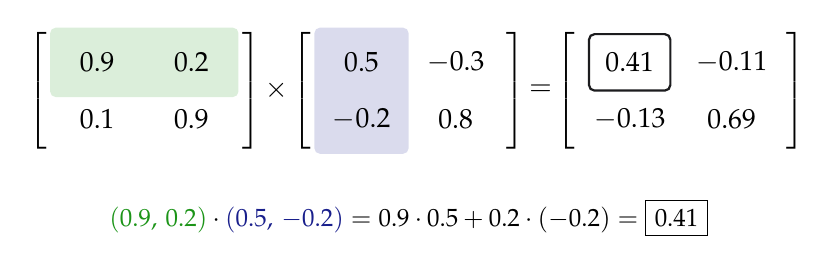
\begin{tikzpicture}[baseline]
  \matrix[matw] (X) { 0.9 \& 0.2 \\ 0.1 \& 0.9 \\ };
  \node[right=6pt of X] (t) {$\times$};
  \matrix[matw,right=6pt of t] (W) { 0.5 \& -0.3 \\ -0.2 \& 0.8 \\ };
  \node[right=6pt of W] (e) {$=$};
  \matrix[matw,right=6pt of e] (Y) { 0.41 \& -0.11 \\ -0.13 \& 0.69 \\ };
  \begin{scope}[on background layer]
    \node[fill=mixink!16, rounded corners=2pt, fit=(X-1-1)(X-1-2)] {};
    \node[fill=measink!16, rounded corners=2pt, fit=(W-1-1)(W-2-1)] {};
  \end{scope}
  \node[draw=ink, line width=0.8pt, rounded corners=2pt, inner sep=1pt, fit=(Y-1-1)] {};
  \node[below=13pt of W, font=\small]
    {$\mix{(0.9,\,0.2)}\cdot\meas{(0.5,\,-0.2)} = 0.9\cdot0.5 + 0.2\cdot(-0.2) = \boxed{0.41}$};
\end{tikzpicture}
\figcap{\textbf{The defining rule.} The entry $Y_{ij}$ is the dot product of the $i$-th \mix{row} of $X$ with the $j$-th \meas{column} of $W$.}
\end{center}

That is the whole operation, and the matrix product $Y$ is now settled. What remains is not to compute it but to read it. The one sum $Y_{ij}=\sum_k X_{ik}W_{kj}$ can be grouped by holding the column index fixed or by holding the row index fixed, and those two groupings become the two readings we develop next.

%============================================================================
\subsection*{Reading 1: measurement (by columns of $W$)}

Fix a column index $j$ and write $\mathbf{w}_j$ for the $j$-th column of $W$. Now gather the entries of column $j$ of $Y$: that column holds the dot product of every input (the rows of $X$) against the single vector $\mathbf{w}_j$. Reading the product this way, scoring each input against each column, we call \meas{measurement}.

\[
Y_{\cdot j} \;=\; X\mathbf{w}_j \;\in\;\mathbb{R}^{n},
\qquad
\bigl(Y_{\cdot j}\bigr)_i \;=\; Y_{ij}\;=\; \mathbf{x}_i\cdot\mathbf{w}_j
\]

\begin{center}
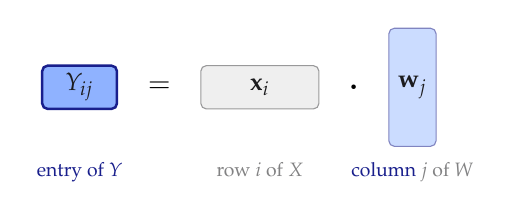
\begin{tikzpicture}[
   xstrip/.style={rounded corners=2pt, draw=ink!45, fill=ink!7, text=ink, minimum width=1.5cm, minimum height=0.55cm, font=\small, inner sep=1pt},
   wcol/.style={rounded corners=2pt, draw=measink!55, fill=measfill, text=ink, minimum width=0.6cm, minimum height=1.5cm, font=\small, inner sep=1pt},
   abox/.style={rounded corners=2pt, draw=measink, line width=0.9pt, fill=measfillb, text=ink, minimum width=0.95cm, minimum height=0.55cm, font=\small, inner sep=1pt}]
  \node[abox] (yij) {$Y_{ij}$};
  \node[right=2.5mm of yij] (eq) {$=$};
  \node[xstrip, right=2.5mm of eq] (x) {$\mathbf{x}_i$};
  \node[right=2.5mm of x] (dot) {$\boldsymbol{\cdot}$};
  \node[wcol, right=2.5mm of dot] (w) {$\mathbf{w}_j$};
  \coordinate (base) at ([yshift=-2pt]w.south);
  \node[font=\scriptsize, measink, anchor=north] at (yij|-base) {entry of $Y$};
  \node[font=\scriptsize, softgray, anchor=north] at (x|-base) {row $i$ of $X$};
  \node[font=\scriptsize, softgray, anchor=north] at (w|-base) {\meas{column} $j$ of $W$};
\end{tikzpicture}
\figcap{\textbf{Measurement: an entry is a score against a column.} Entry $Y_{ij}$ is the dot product of input~$i$ --- the $i$-th row of $X$ --- with the \meas{$j$-th column} of $W$, measuring how far that input reaches along the direction $\mathbf{w}_j$. Each column poses its own question, and the matching column of $Y$ collects every input's score.}
\end{center}

What is $\mathbf{w}_j$ doing here? It is a \emph{vector} in feature space, the same $\mathbb{R}^{d}$ the inputs live in. Picture it as an arrow from the origin, carrying both a length and a way of pointing. What matters about this arrow is almost entirely the way it points, its \emph{direction}. To score an input against $\mathbf{w}_j$ is to ask how far the input reaches \emph{along} that direction. The input's perpendicular shadow on the line through $\mathbf{w}_j$ --- its \emph{projection} --- makes that reach visible, and the dot product reports it as a single number, positive when the shadow runs forward, negative when it falls backward. The arrow's length, by contrast, plays no role in the comparison. It sets only the units the scores are reported in: stretching $\mathbf{w}_j$ multiplies every input's score by the same factor, so the ranking of the inputs, and the sign of each, are left exactly as they were. So a column of $W$ fixes a direction in feature space, and the matching column of $Y$ records how far each input extends along that direction.

To make this concrete, let's look at the figure below. The two inputs \meas{$\mathbf{x}_1$} and \meas{$\mathbf{x}_2$} sit in feature space, and $\mathbf{w}_1=(0.5,-0.2)$ fixes a direction, the dashed green line through it. Dropping each input perpendicularly onto that line gives its projection: $\mathbf{x}_1$ scores $\mathbf{x}_1\cdot\mathbf{w}_1 = 0.9\cdot0.5+0.2\cdot(-0.2) = 0.41$, while $\mathbf{x}_2$ scores $-0.13$. The length and sign of each shadow are just \emph{alignment} made visible: $\mathbf{x}_1$ makes a small angle with $\mathbf{w}_1$ and so points much the same way, its shadow running forward; $\mathbf{x}_2$ makes an angle past a right angle and so points partly against $\mathbf{w}_1$, its shadow falling backward and its score turning negative. This is exactly $\mathbf{x}\cdot\mathbf{w}_1=\lVert\mathbf{x}\rVert\,\lVert\mathbf{w}_1\rVert\cos\theta$ at work. The narrower the angle, the larger $\cos\theta$, and the longer the forward projection. Those two numbers are precisely the first column of $Y$.

\begin{center}
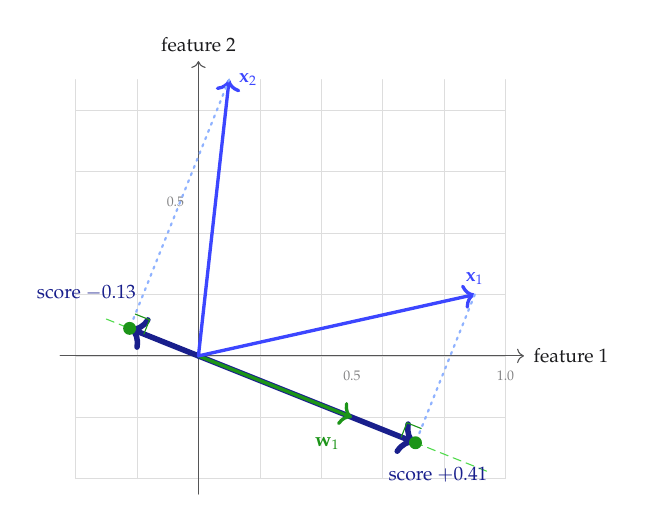
\begin{tikzpicture}[scale=3.9, line cap=round]
  \draw[step=0.2, ink!15, very thin] (-0.4,-0.4) grid (1.0,0.9);
  \draw[->, ink!75] (-0.45,0) -- (1.06,0) node[right,ink,font=\scriptsize]{feature 1};
  \draw[->, ink!75] (0,-0.45) -- (0,0.96) node[above,ink,font=\scriptsize]{feature 2};
  \node[font=\tiny,ink!55] at (0.5,-0.065){0.5};
  \node[font=\tiny,ink!55] at (1.0,-0.065){1.0};
  \node[font=\tiny,ink!55] at (-0.075,0.5){0.5};
  \draw[densely dashed, grnBright] (-0.30,0.12) -- (0.95,-0.38);
  \draw[->, line width=2pt, bluDark] (0,0) -- (0.7069,-0.2828);
  \draw[->, line width=2pt, bluDark] (0,0) -- (-0.2241,0.0897);
  \draw[->, very thick, grnMed] (0,0) -- (0.5,-0.2);
  \node[grnMed,font=\scriptsize] at (0.42,-0.285) {$\mathbf{w}_1$};
  \draw[->, very thick, bluBright] (0,0) -- (0.9,0.2);
  \node[bluBright,font=\scriptsize,above] at (0.9,0.2) {$\mathbf{x}_1$};
  \draw[->, very thick, bluBright] (0,0) -- (0.1,0.9);
  \node[bluBright,font=\scriptsize,right] at (0.1,0.9) {$\mathbf{x}_2$};
  \draw[dotted, bluLight, thick] (0.9,0.2) -- (0.7069,-0.2828);
  \draw[dotted, bluLight, thick] (0.1,0.9) -- (-0.2241,0.0897);
  \draw[grnMed, line width=0.4pt] (0.6605,-0.2642)--(0.6791,-0.2178)--(0.7255,-0.2364);
  \draw[grnMed, line width=0.4pt] (-0.1777,0.0711)--(-0.1591,0.1175)--(-0.2055,0.1361);
  \fill[grnMed] (0.7069,-0.2828) circle (0.6pt);
  \fill[grnMed] (-0.2241,0.0897) circle (0.6pt);
  \node[bluDark,font=\scriptsize] at (0.78,-0.385) {score $+0.41$};
  \node[bluDark,font=\scriptsize] at (-0.365,0.205) {score $-0.13$};
\end{tikzpicture}
\figcap{\textbf{Measurement as projection.} Each input casts a perpendicular shadow onto the line through $\mathbf{w}_1$, and the thick arrow on that line is the projection itself. The labels give each input's \emph{score} $\mathbf{x}\cdot\mathbf{w}_1$, proportional to the shadow's signed length.}
\end{center}



%============================================================================
\subsection*{Reading 2: mixing (by rows of $W$)}

Fix instead a row index $i$, and write $\mathbf{r}_k\in\mathbb{R}^{m}$ for the $k$-th row of $W$. The $i$-th row of $Y$ is then a \emph{linear combination} of the rows of $W$ whose coefficients are the entries of the $i$-th row of $X$. Reading the product this way, building each output row by combining the rows of $W$, we call \mix{mixing}.

\[
Y_{i\cdot} \;=\; \sum_{k=1}^{d} X_{ik}\,\mathbf{r}_k \;\in\;\mathbb{R}^{m}
\]

\begin{center}
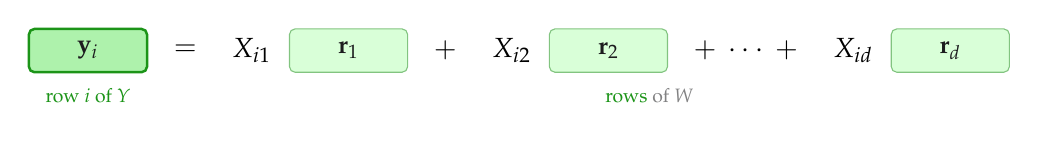
\begin{tikzpicture}[
   vstrip/.style={rounded corners=2pt, draw=mixink!55, fill=mixfill, text=ink, minimum width=1.5cm, minimum height=0.55cm, font=\small, inner sep=1pt},
   hstrip/.style={rounded corners=2pt, draw=mixink, line width=0.9pt, fill=mixfillb, text=ink, minimum width=1.5cm, minimum height=0.55cm, font=\small, inner sep=1pt}]
  \node[hstrip] (y) {$\mathbf{y}_i$};
  \node[right=2mm of y] (eq) {$=$};
  \node[right=2mm of eq] (a1) {$X_{i1}$};
  \node[vstrip, right=1mm of a1] (r1) {$\mathbf{r}_1$};
  \node[right=2mm of r1] (p1) {$+$};
  \node[right=2mm of p1] (a2) {$X_{i2}$};
  \node[vstrip, right=1mm of a2] (r2) {$\mathbf{r}_2$};
  \node[right=2mm of r2] (p2) {$+\ \cdots\ +$};
  \node[right=2mm of p2] (ad) {$X_{id}$};
  \node[vstrip, right=1mm of ad] (rd) {$\mathbf{r}_d$};
  \node[font=\scriptsize, mixink, below=2pt of y] {row $i$ of $Y$};
  \node[font=\scriptsize, softgray, anchor=north] at ([yshift=-2pt]$(r1.south)!0.5!(rd.south)$) {\mix{rows} of $W$};
\end{tikzpicture}
\figcap{\textbf{Mixing: an output row is a blend of $W$'s rows.} Row~$i$ of $Y$ is a weighted combination of the \mix{rows} of $W$, $\mathbf{r}_1,\dots,\mathbf{r}_d$, with weights $X_{i1},\dots,X_{id}$ read off row~$i$ of $X$. The rows are shared by every input; only the weights change from one input to the next, so each output row is its own blend of the same $d$ rows.}
\end{center}

The rows of $W$ are a fixed handful of vectors in the \emph{output} space $\mathbb{R}^m$, shared by every input. To take a linear combination of them is to scale each by some amount and add the results, and the output for input~$i$ is one such combination, $X_{i1}\,\mathbf{r}_1+X_{i2}\,\mathbf{r}_2+\cdots+X_{id}\,\mathbf{r}_d$. As the coefficients range over all values, \emph{positive and negative}, such combinations sweep out the \emph{span} of $\mathbf{r}_1,\dots,\mathbf{r}_d$, the entire region of points they can reach. As long as the rows point in genuinely different directions, as our two do, that region is the whole of $\mathbb{R}^m$ whenever there are at least $m$ of them; in general it is the subspace they span. Every output the map can ever produce is some blend of the same $d$ rows, with the input's entries setting how much of each to take.

On the running example, $\mathbf{r}_1=(0.5,-0.3)$ and $\mathbf{r}_2=(-0.2,0.8)$, and
\[
Y_{1\cdot}=0.9\,\mathbf{r}_1+0.2\,\mathbf{r}_2=(0.41,-0.11),
\qquad
Y_{2\cdot}=0.1\,\mathbf{r}_1+0.9\,\mathbf{r}_2=(-0.13,0.69).
\]
The two rows ($\mathbf{r}_1, \mathbf{r}_2$) are common to both outputs; only the amounts, read off each input's row, change. 

\begin{center}
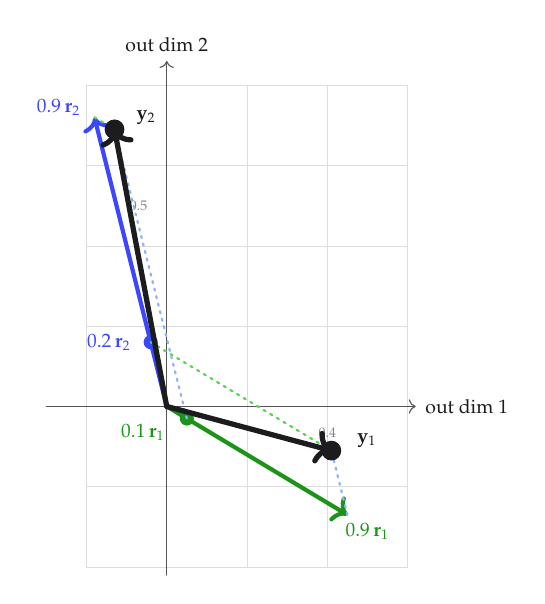
\begin{tikzpicture}[scale=5.1, line cap=round]
  \draw[step=0.2, ink!15, very thin] (-0.2,-0.4) grid (0.6,0.8);
  \draw[->, ink!75] (-0.30,0) -- (0.62,0) node[right,font=\scriptsize,ink]{out dim 1};
  \draw[->, ink!75] (0,-0.42) -- (0,0.86) node[above,font=\scriptsize,ink]{out dim 2};
  \node[font=\tiny,ink!55] at (0.4,-0.065){0.4};
  \node[font=\tiny,ink!55] at (-0.07,0.5){0.5};
  \draw[->, line width=1.5pt, grnMed]  (0,0) -- (0.45,-0.27);
  \draw[->, line width=1.5pt, bluBright] (0,0) -- (-0.18,0.72);
  \fill[grnMed]  (0.05,-0.03) circle (0.5pt);
  \fill[bluBright] (-0.04,0.16) circle (0.5pt);
  \draw[dotted, bluLight,  thick] (0.45,-0.27) -- (0.41,-0.11);
  \draw[dotted, grnBright, thick] (-0.04,0.16) -- (0.41,-0.11);
  \draw[dotted, bluLight,  thick] (0.05,-0.03) -- (-0.13,0.69);
  \draw[dotted, grnBright, thick] (-0.18,0.72) -- (-0.13,0.69);
  \draw[->, line width=1.9pt, ink] (0,0) -- (0.41,-0.11);
  \draw[->, line width=1.9pt, ink] (0,0) -- (-0.13,0.69);
  \fill[ink] (0.41,-0.11) circle (0.7pt);
  \fill[ink] (-0.13,0.69) circle (0.7pt);
  \node[grnMed,font=\scriptsize,left]    at (0.02,-0.065) {$0.1\,\mathbf{r}_1$};
  \node[bluBright,font=\scriptsize,left]  at (-0.065,0.16) {$0.2\,\mathbf{r}_2$};
  \node[grnMed,font=\scriptsize]          at (0.50,-0.31) {$0.9\,\mathbf{r}_1$};
  \node[bluBright,font=\scriptsize,left]  at (-0.19,0.745) {$0.9\,\mathbf{r}_2$};
  \node[ink,font=\scriptsize,right]       at (0.45,-0.085) {$\mathbf{y}_1$};
  \node[ink,font=\scriptsize,right]       at (-0.10,0.72) {$\mathbf{y}_2$};
\end{tikzpicture}
\figcap{\textbf{Mixing: a blend of $W$'s two rows.} Each output is a linear combination of the two rows of $W$, each row scaled by the input's entries and added. Because the two rows span the output plane, every reachable output is some such blend.}
\end{center}

%============================================================================
\subsection*{The two readings coincide}

Why two readings of one product, and why are they drawn in different spaces? Because the same matrix $W$ meets the two readings through different slices. A \emph{column} of $W$ has $d$ entries, one for each input feature, so it is a vector in the input space $\mathbb{R}^{d}$, sitting among the inputs; that is the space the measurement figure is drawn in, and a column is something an input can be measured \emph{against}. A \emph{row} of $W$ has $m$ entries, one for each output dimension, so it is a vector in the output space $\mathbb{R}^{m}$, sitting among the outputs; that is the space the mixing figure is drawn in, and a row is something an output can be built \emph{from}.

Whichever reading we take, the arithmetic beneath it is the same. Pick any entry $Y_{ij}$. Measurement reaches it by pairing input $i$ with column $j$; mixing reaches it as the $j$-th coordinate of the blend that forms output $i$. Both come out to the one sum $Y_{ij}=\sum_{k}X_{ik}W_{kj}$. There is really a single matrix product $Y$: read it column by column and it tells the measurement story, read it row by row and it tells the mixing story.

% \begin{center}
% \begin{tikzpicture}[node distance=6mm]
%   \node[draw=ink, line width=1pt, rounded corners=3pt, minimum width=15mm,
%         minimum height=11mm, font=\large\bfseries] (val) {$0.41$};
%   \node[left=26mm of val, align=center, draw=measink, rounded corners=2pt,
%         fill=measink!8, inner sep=5pt, font=\small, text width=3.5cm] (L)
%     {\meas{measurement}\\[2pt] $\mathbf{x}_1 \cdot \mathbf{w}_1$};
%   \node[right=26mm of val, align=center, draw=mixink, rounded corners=2pt,
%         fill=mixink!8, inner sep=5pt, font=\small, text width=3.6cm] (R)
%     {\mix{mixing}\\[2pt] coord.\ $1$ of $0.9\,\mathbf{r}_1+0.2\,\mathbf{r}_2$};
%   \draw[arr, measink] (L.east) -- (val.west);
%   \draw[arr, mixink] (R.west) -- (val.east);
%   \node[below=9mm of val, font=\small] (s)
%     {same sum:\;\; $0.9\cdot0.5 + 0.2\cdot(-0.2)$};
%   \draw[arr, ink] (s.north) -- (val.south);
% \end{tikzpicture}
% \figcap{\textbf{One entry, two derivations.} Measurement reaches $Y_{11}=0.41$ as the dot product $\mathbf{x}_1\cdot\mathbf{w}_1$; mixing reaches it as the first coordinate of $0.9\,\mathbf{r}_1+0.2\,\mathbf{r}_2$. Both reduce to the same sum.}
% \end{center}

We carry both forward, under the names \meas{measurement} and \mix{mixing}, for the rest of the document.

\subsection*{Neural Networks in Essence}

So far $W$ has simply been given to us. In a neural network its entries are \emph{learned}. This is what the name \emph{machine learning} refers to, a machine that learns its own weights. The learning follows one loop. The network makes a prediction, compares it with the truth, and measures the gap as an error. An algorithm called \emph{backpropagation} then traces the error backwards through the network, working out how much each weight contributed and in which direction a small correction would help. Over millions of examples the corrections accumulate, and the weights settle into values that serve the task. (The full mechanics are beyond our scope; the videos of Appendix~A treat them properly.)

Machine learning (ML) papers frequently say a weight matrix ``projects'' inputs into a
learned space. The original transformer paper by Vaswani et al.\
\citeyearpar{vaswani2017attention}, for instance, speaks of mapping the
queries, keys, and values with ``different, learned linear projections'',
and later writing often describes $W_Q$, $W_K$, $W_V$ as projection
matrices carrying embeddings into an attention space. In ML, ``projection'' usually means \textit{some} linear
transformation, that is, multiplying by a weight matrix to produce a new
representation.

Consider $Y = XW$ where $W$ has shape $d \times m$. We say $W$ ``projects''
$d$-dimensional inputs into an $m$-dimensional learned space, learned because the
entries of $W$ are fixed by training. The \meas{columns} of $W$ become directions
that detect meaningful patterns, and its \mix{rows} become templates that blend
together. Whether $m$ is smaller than $d$, larger, or equal, the key idea is that $W$ re-expresses inputs in terms of
patterns this nudging has discovered to be useful for the task.

This \textit{is} the building block of deep learning. A neural network chains
these projections with nonlinearities, so that each layer applies
$\mathbf{y} = f(XW + \mathbf{b})$, projecting into a new learned space via $XW$
and then bending\footnote{%
Bending means reshaping the space in ways a matrix cannot. On its own, matrix
multiplication can only rotate, stretch, and shear the space (i.e., straight lines
stay straight). A \emph{nonlinearity} is a simple, fixed rule applied to each
number on its own --- for instance ReLU, which replaces every negative value
with zero, or the sigmoid, which squashes every value into the range from $0$ to
$1$. Rules like these bend the space, adding the curves, folds, and corners a
matrix never could. This is essential because real-world patterns are rarely linearly separable. Bending allows the network to curve decision boundaries around complex patterns, transforming messy, entangled data into spaces where simple linear separators work.} it with the nonlinearity $f$. The nonlinearity is what
makes depth meaningful. Without it, stacking layers gains nothing, since
$(XW_1)W_2 = X(W_1 W_2)$ collapses to a single linear transformation no matter
how many layers we pile up. The nonlinearity is what preserves the hierarchy
that depth creates.

The power of deep networks comes from iterating this loop, projecting into a
learned space, bending through a nonlinearity, and projecting again. Layer~1
might project into a space where primitive features emerge, layer~2 into a space
where combinations of those primitives become visible, layer~3 into a space
where higher abstractions make sense. Each cycle refines what the network
``sees'' in the data, building from raw measurements towards abstract
understanding.

\paragraph{A Note on Parallelisation} To \textit{parallelise} a computation is to perform many of its parts at the same time rather than one after another. Matrix multiplication is a natural candidate, because the entries of $Y$ do not depend on one another. Computing any single entry $y_{ij}$ needs only row~$i$ of $X$ and column~$j$ of $W$, so all entries can be worked out simultaneously, in any order, on separate hardware. In the transformer setting, though, parallelisation carries a second and more consequential meaning, the removal of \textit{sequential dependencies} across the sequence. Before transformers, the dominant tool for sequences was the recurrent neural network (RNN), which read a sequence strictly in order, token~1, then token~2, then token~3, because each hidden state was built from the one before it. That was an unavoidable bottleneck, no matter how parallelisable the underlying matrix multiplications happened to be. Transformers remove it by processing all tokens in a sequence at once within each layer, with no position waiting on any other. This single architectural change was a major factor in making training on far larger datasets and models practical.

\paragraph{Row Convention} Throughout this document, we represent samples (or token embeddings) as \textit{row vectors}, not column vectors. Linear algebra textbooks typically use column vectors, but ML conventionally uses row vectors, with two practical reasons. The first is memory layout. In row-major storage (used by C, Python/NumPy, and PyTorch), the $d$ entries of a row sit contiguously in memory, so a token stored as a row of an $(n, d)$ matrix occupies one contiguous block. The second is readability. With row vectors the forward pass reads left to right as \texttt{x @ W1 @ W2 @ W3}, matching both reading order and the conceptual flow through the layers. Neither point makes the convention necessary. The identical computation can be written with column vectors, and the difference is one of convention and convenience rather than of what the network can express.

\subsection*{From Features to Word Vectors}

Before we close this section, one matrix deserves a final look. Of the three in $Y = XW$, we know by now where two come from. $Y$ is computed, and $W$ is learned. Only $X$ has been handed to us from outside, as numbers that someone measured and wrote down. This note, however, is about language models, whose inputs are words. Each word must somehow become a vector, and in an LLM that vector is not designed but \emph{learned}, exactly as the weights are. The inputs, then, come out of training too, as numbers that were never measurements of anything. If nothing was measured, what do the entries record? Before facing that question for learned vectors, let's recall how meaning entered the numbers when we chose them ourselves.

A \emph{feature}, we said, is a property an input can have \citep{elhage2022toy}, a fact about the world, with its coordinate recording how much. When a dataset records each day's weather as (temperature, humidity), \emph{we} decided what the axes mean, and reading a feature off an input is just reading a coordinate. In settings like these the input space is transparent, because every axis was chosen by hand.

However, text breaks this arrangement. What are the features of the word \textit{meaning}? Its abstractness, its life as noun and as verb, the company it keeps, the shade it takes on in \textit{well-meaning} or in \textit{the meaning of life}. The list is real but unbounded, and nobody can sit down and assign each entry an axis. Fortunately, the field has discovered that they can be \emph{learned}. A method called word2vec \citep{mikolov2013efficient} trained small networks on enormous amounts of text with a simple objective, predicting each word from the words around it, and in doing so gave every word in the vocabulary its own vector. No axis was ever told what to mean. Yet when training ended, meaning had appeared in the geometry \citep{mikolov2013linguistic}:
\[
\mathrm{vec}(\textit{king}) - \mathrm{vec}(\textit{man}) + \mathrm{vec}(\textit{woman}) \;\approx\; \mathrm{vec}(\textit{queen}).
\]
Subtracting $\mathrm{vec}(\textit{man})$ removes the part of \textit{king} that points along one particular direction, and adding $\mathrm{vec}(\textit{woman})$ writes in another. That the result lands near \textit{queen} tells us that these directions, in some sense, \emph{represent} features. Gender and royalty are properties of words, facts about the world, and this space has encoded each one along a direction of its own.

The \emph{linear representation hypothesis} holds that many meaningful features, concepts among them, are represented inside a neural network as approximately linear directions in its learned space. Take two words that are alike except in one feature, such as \textit{man} and \textit{woman}, and subtract their vectors. What is left is a shift, the change that turns one vector into the other. The hypothesis says that this shift is roughly the same for every such pair, from \textit{king} to \textit{queen}, from \textit{uncle} to \textit{aunt}, and that shared shift is the gender \emph{direction}. The arithmetic above did nothing more than take \textit{king} and apply the \textit{man}-to-\textit{woman} shift.

Now let's look at what a shift is made of. Vectors subtract entry by entry, so the gender shift is a list of $d$ changes, one per entry. What matters is how those changes are spread across the entries, and the spreading runs both ways. One feature reaches many entries, because no axis was ever told what to mean. One entry is reached by many features, and it keeps only their total. So a feature cannot be read from one entry, and an entry cannot be traced back to a feature; what carries the feature is the whole list of $d$ changes at once, which is the shift, the direction. Meaning, then, lies not in the entries but in the directions that run across them.

\bigskip

With measurement, mixing, and projection in hand, and with meaning now attached to the numbers, we have the whole vocabulary we need. Every operation in a transformer, however imposing its notation, turns out to be one of these moves repeated and recombined. Before examining those operations one at a time, the next section steps back to show the entire machine at once: how tokens become embeddings, how layers stack, how attention and feedforward networks interleave, and where the predictions finally emerge. With that map in view, each later section can zoom in on a single component.

\newpage
\section{Language Model in a Nutshell}
%==============================================================================

In a nutshell, an LLM is a stack of transformer blocks. And each block is simply a chain of matrix operations. Before diving into the mathematics, let's see what this chain looks like.

\begin{center}
\resizebox{\textwidth}{!}{%
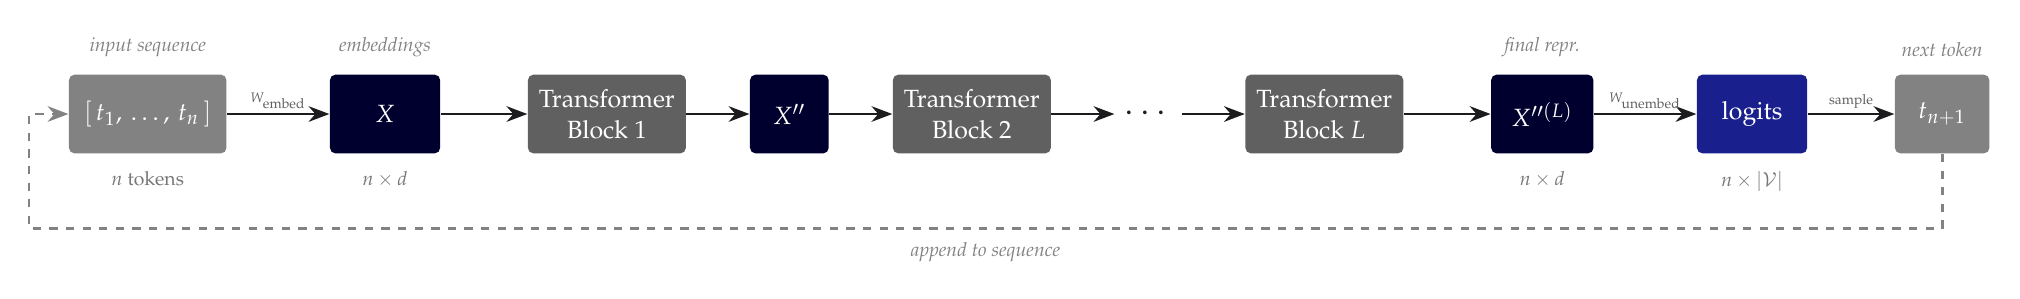
\begin{tikzpicture}[node distance=0.6cm]
  \node[sToken, minimum width=2.0cm, minimum height=1.0cm] (tokens) {$[\,t_1,\,\ldots,\,t_n\,]$};
  \node[sDim, below=0.1cm of tokens] {$n$ tokens};
  \node[sLbl, above=0.1cm of tokens] {input sequence};
  \node[sData, right=1.3cm of tokens, minimum width=1.4cm, minimum height=1.0cm] (X) {$X$};
  \node[sDim, below=0.1cm of X] {$n \times d$};
  \node[sLbl, above=0.1cm of X] {embeddings};
  \draw[sArrow] (tokens) -- node[sEdge, above] {$W_{\text{embed}}$} (X);
  \node[sLayer, right=1.1cm of X, minimum width=2.0cm, minimum height=1.0cm] (L1) {Transformer\\Block 1};
  \draw[sArrow] (X) -- (L1);
  \node[sData, right=0.8cm of L1, minimum width=1.0cm, minimum height=1.0cm] (X1) {$X''$};
  \draw[sArrow] (L1) -- (X1);
  \node[sLayer, right=0.8cm of X1, minimum width=2.0cm, minimum height=1.0cm] (L2) {Transformer\\Block 2};
  \draw[sArrow] (X1) -- (L2);
  \node[right=0.8cm of L2, font=\large, text=ink] (dots) {$\cdots$};
  \draw[sArrow] (L2) -- (dots);
  \node[sLayer, right=0.8cm of dots, minimum width=2.0cm, minimum height=1.0cm] (LL) {Transformer\\Block $L$};
  \draw[sArrow] (dots) -- (LL);
  \node[sData, right=1.1cm of LL, minimum width=1.3cm, minimum height=1.0cm] (Xfinal) {$X''^{(L)}$};
  \node[sDim, below=0.1cm of Xfinal] {$n \times d$};
  \node[sLbl, above=0.1cm of Xfinal] {final repr.};
  \draw[sArrow] (LL) -- (Xfinal);
  \node[sBlue, right=1.3cm of Xfinal, minimum width=1.4cm, minimum height=1.0cm] (logits) {logits};
  \node[sDim, below=0.1cm of logits] {$n \times |\mathcal{V}|$};
  \draw[sArrow] (Xfinal) -- node[sEdge, above] {$W_{\text{unembed}}$} (logits);
  \node[sToken, right=1.1cm of logits, minimum width=1.2cm, minimum height=1.0cm] (next) {$t_{n+1}$};
  \node[sLbl, above=0.1cm of next] {next token};
  \draw[sArrow] (logits) -- node[sEdge, above] {sample} (next);
  \coordinate (fbr) at ($(next.south) + (0, -0.95)$);
  \coordinate (fbw) at ($(tokens.west) + (-0.5, 0)$);
  \path let \p1=(fbr) in coordinate (fbl) at (fbw |- \p1);
  \draw[sFeedback] (next.south) -- (fbr) -- (fbl) -- (fbw) -- (tokens.west);
  \node[sLbl, below=0.05cm] at ($(fbl)!0.5!(fbr)$) {append to sequence};
\end{tikzpicture}}
\vspace{0.3em}

{\small \textbf{Figure 1:} LLM Pipeline (High-Level)}
\end{center}

LLMs take a sequence of tokens as input, convert each token into an embedding vector, and pass these through a stack of transformer blocks which build progressively richer, contextualised representations of meaning (Figure~1). The final representation of the last token then produces a score for every token in the vocabulary, the \emph{logits}, which a final step turns into a probability distribution over possible next tokens. The model samples from this distribution, appends the chosen token to the input, and repeats; predicting the next token, one at a time.

Each transformer block is a multi-layer network consisting of attention, feedforward, normalisation layers, and residual connections. In Figure~2a, the residual pathway from $X$ to $X''$ is drawn as a straight central line, the \textit{residual stream}, with attention and the feedforward network branching off it, doing their work, and adding their results back in. Seen this way, each sublayer \emph{reads} from the stream and \emph{writes} its result back.

\begin{center}
\resizebox{\textwidth}{!}{%
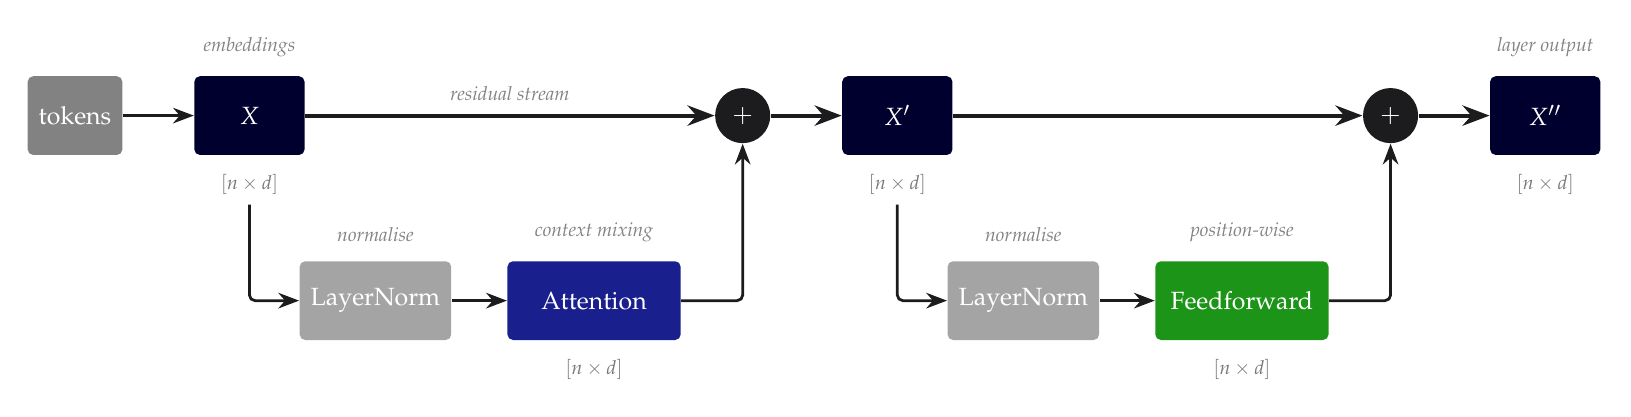
\begin{tikzpicture}[node distance=0.6cm]
  % ---- the residual stream: a straight center line from X to X'' ----
  \node[sToken, minimum width=1.2cm, minimum height=1.0cm] (tokens) {tokens};
  \node[sData, right=0.9cm of tokens, minimum width=1.4cm, minimum height=1.0cm] (X) {$X$};
  \node[sDim, below=0.12cm of X] (Xdim) {$[n \times d]$};
  \node[sLbl, above=0.12cm of X] {embeddings};
  \draw[sArrow] (tokens) -- (X);
  \node[sOp, right=5.2cm of X] (add1) {$+$};
  \node[sData, right=0.9cm of add1, minimum width=1.4cm, minimum height=1.0cm] (Xmid) {$X'$};
  \node[sDim, below=0.12cm of Xmid] (Xmiddim) {$[n \times d]$};
  \node[sOp, right=5.2cm of Xmid] (add2) {$+$};
  \node[sData, right=0.9cm of add2, minimum width=1.4cm, minimum height=1.0cm] (Xout) {$X''$};
  \node[sDim, below=0.12cm of Xout] {$[n \times d]$};
  \node[sLbl, above=0.12cm of Xout] {layer output};
  \draw[sStream] (X) -- (add1);
  \draw[sStream] (add1) -- (Xmid);
  \draw[sStream] (Xmid) -- (add2);
  \draw[sStream] (add2) -- (Xout);
  \node[sLbl, above=0.06cm] at ($(X.east)!0.5!(add1.west)$) {residual stream};
  % ---- attention sublayer: branches off the stream, adds back at + ----
  \node[sNorm, minimum width=1.6cm, minimum height=1.0cm] (LN1) at ($(X.center)+(1.6,-2.35)$) {LayerNorm};
  \node[sLbl, above=0.12cm of LN1] {normalise};
  \node[sBlue, right=0.7cm of LN1, minimum width=2.2cm, minimum height=1.0cm] (attn) {Attention};
  \node[sDim, below=0.12cm of attn] {$[n \times d]$};
  \node[sLbl, above=0.12cm of attn] {context mixing};
  \draw[sArrow, rounded corners=2pt] (Xdim.south) |- (LN1.west);
  \draw[sArrow] (LN1) -- (attn);
  \draw[sArrow, rounded corners=2pt] (attn.east) -| (add1.south);
  % ---- feedforward sublayer: branches off the stream, adds back at + ----
  \node[sNorm, minimum width=1.6cm, minimum height=1.0cm] (LN2) at ($(Xmid.center)+(1.6,-2.35)$) {LayerNorm};
  \node[sLbl, above=0.12cm of LN2] {normalise};
  \node[sGreen, right=0.7cm of LN2, minimum width=2.2cm, minimum height=1.0cm] (FFN) {Feedforward};
  \node[sDim, below=0.12cm of FFN] {$[n \times d]$};
  \node[sLbl, above=0.12cm of FFN] {position-wise};
  \draw[sArrow, rounded corners=2pt] (Xmiddim.south) |- (LN2.west);
  \draw[sArrow] (LN2) -- (FFN);
  \draw[sArrow, rounded corners=2pt] (FFN.east) -| (add2.south);
\end{tikzpicture}}
\vspace{0.3em}

{\small \textbf{Figure 2a:} Transformer Block (High-Level)}
\end{center}

The \textbf{attention layer} builds contextual representations by allowing each token to ``attend'' to and integrate information from surrounding tokens. The \textbf{feedforward layer} is a simple two-layer fully connected neural network that processes the integrated information for each embedding independently, often called position-wise because it operates on each position separately. \textbf{Normalisation layers} support these sublayers, enabling the network to be trained stably at depth.

\newpage
Figure~2b expands one transformer block into its individual operations, tracing how a token's representation flows through each step. It is the most detailed diagram in this document, and it is meant to be returned to. On a first read, do not try to parse every symbol. Instead, follow the flow downward and track one thing, the shape of the data. A representation enters at the top and travels down the residual stream, leaving at the bottom in the same shape ($n \times d$) it arrived, only richer; attention and the feedforward network branch off the stream, compute, and merge what they find back into the stream. The dimensions change only briefly inside the sublayers, both within attention (down to $d_k$ and $d_v$) and within the feedforward network (up to $d_{\text{ff}}$ and back down), before being restored to $[n \times d]$ each time. Every symbol in this figure is unpacked, one operation at a time, in the sections that follow.

\begin{center}
\begin{minipage}[t]{4.5cm}
  \vspace{0pt}
  {\centering
  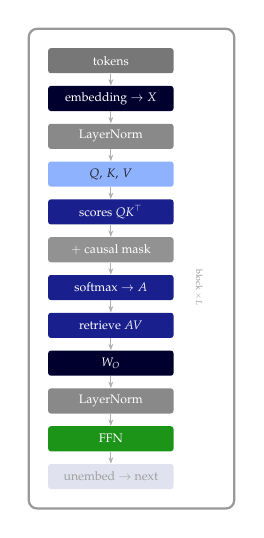
\begin{tikzpicture}
    \node[draw=ink!45, line width=0.8pt, rounded corners=3pt, inner sep=7pt]
      {\resizebox{!}{5.6cm}{\minimap{tokens,embed,ln,qkv,score,mask,soft,ret,heads,ffn}}};
  \end{tikzpicture}\par}
  \vspace{0.7em}
  {\footnotesize\color{softgray} This mini-map returns at each section with the active step lit. Sections~4 to 12 will cover these operations step by step.\par}
\end{minipage}%
\hspace{0.5cm}%
\begin{minipage}[t]{10.4cm}
  \vspace{0pt}\centering
  \resizebox{!}{0.69\textheight}{%
  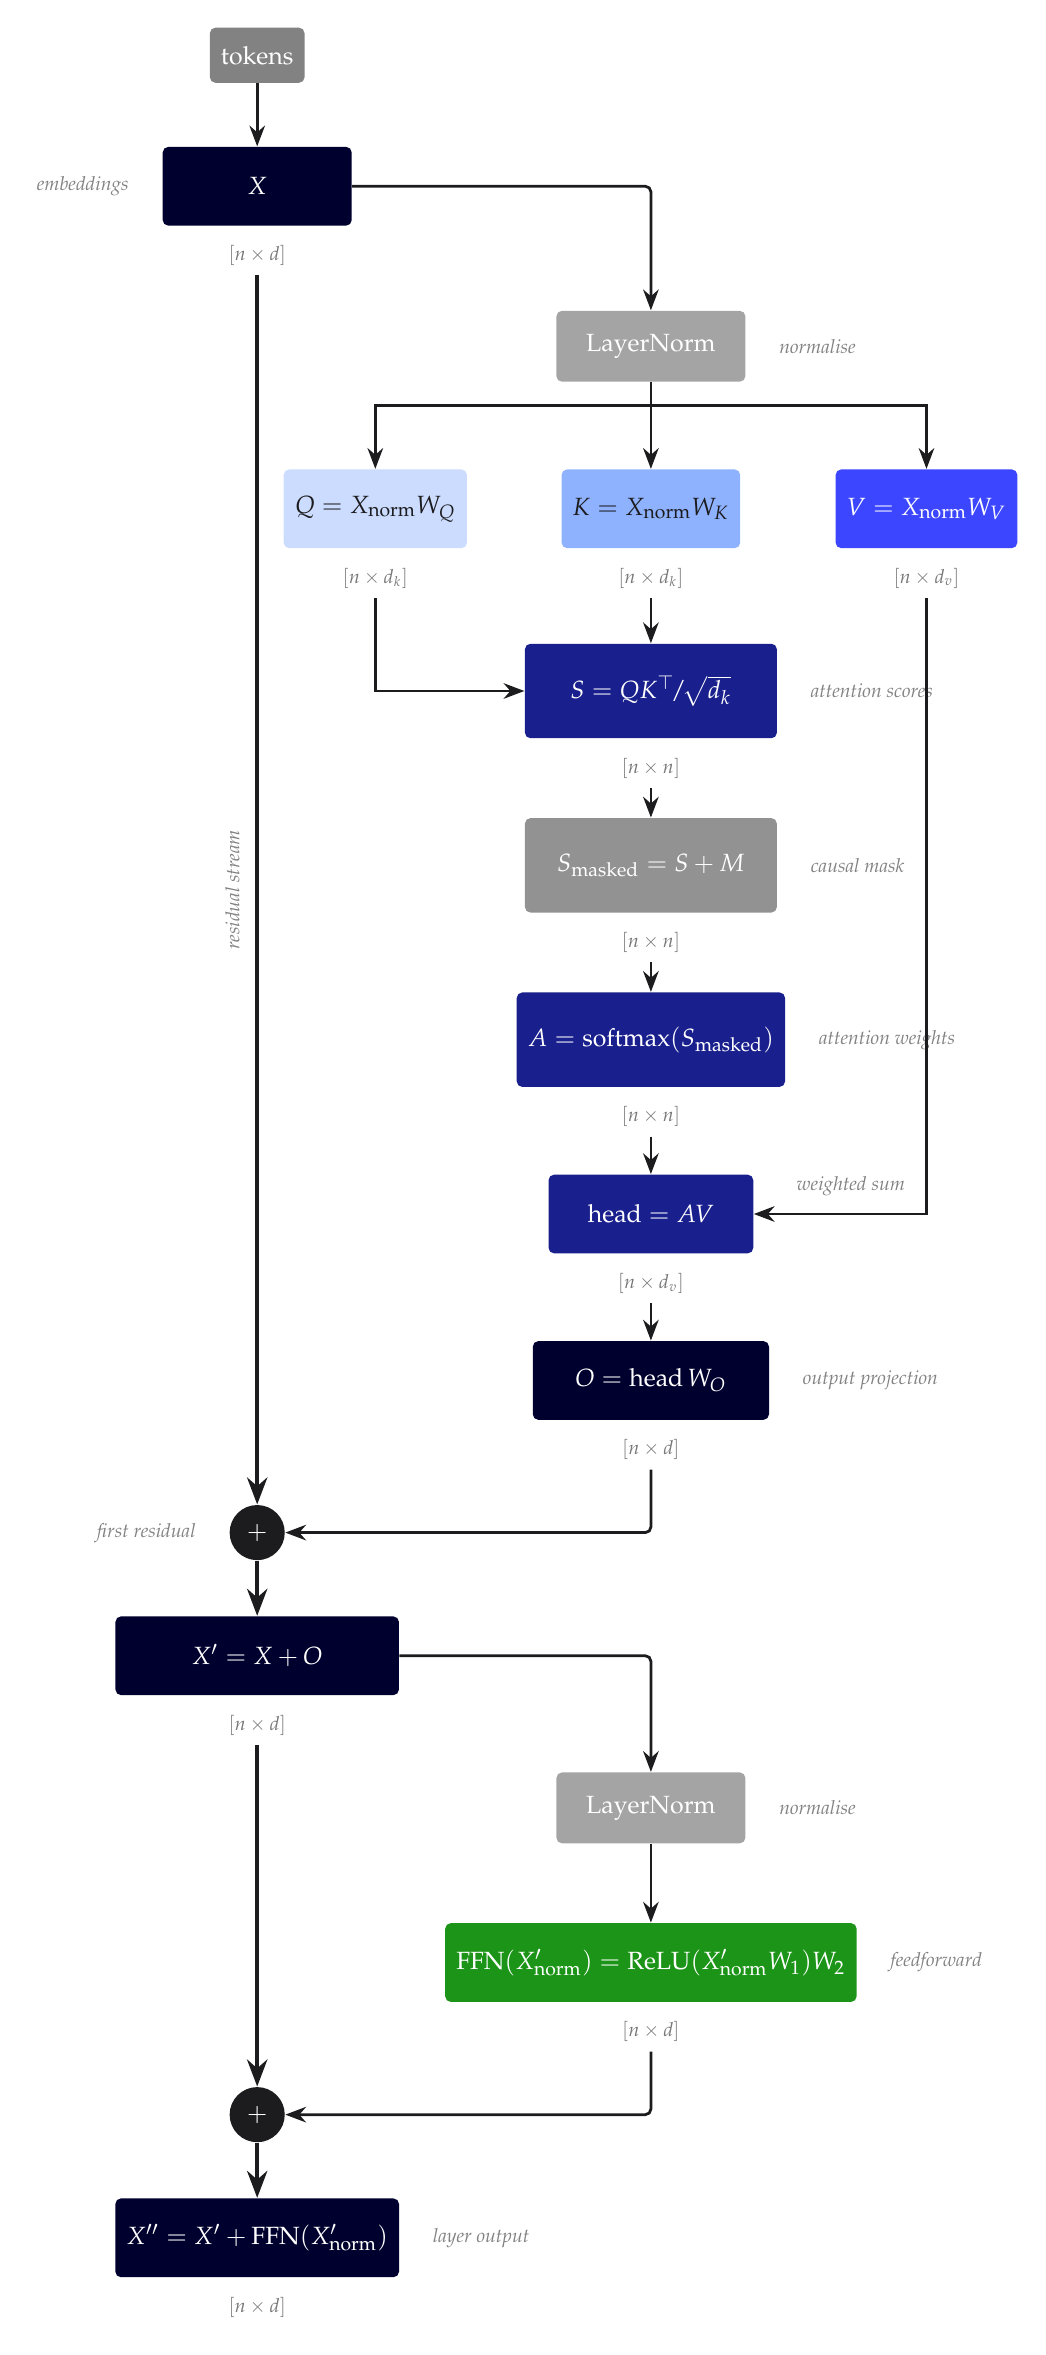
\begin{tikzpicture}[node distance=0.4cm and 0.7cm,
    mnode/.style={fbox, minimum width=2.4cm, minimum height=1.0cm},
   qkv/.style={fbox, minimum width=2.2cm, minimum height=1.0cm},
   formula/.style={fbox, minimum width=3.2cm, minimum height=1.2cm},
   headm/.style={fbox, minimum width=2.6cm, minimum height=1.0cm},
   outm/.style={fbox, minimum width=3.0cm, minimum height=1.0cm},
   resm/.style={fbox, minimum width=3.6cm, minimum height=1.0cm},
   mlpm/.style={fbox, minimum width=4.2cm, minimum height=1.0cm},
   maskm/.style={fbox, minimum width=3.2cm, minimum height=1.2cm},
   normm/.style={fbox, minimum width=2.4cm, minimum height=0.9cm}]
  % ---- residual stream: straight central spine from X down to X'' ----
  \node[sToken, minimum width=1.2cm, minimum height=0.7cm] (tokens) {tokens};
  \node[mnode, sData, below=0.8cm of tokens] (X) {$X$};
  \node[sDim, below=0.12cm of X] (Xdim) {$[n \times d]$};
  \node[sLbl, left=0.3cm of X] {embeddings};
  \draw[sArrow] (tokens) -- (X);
  % ---- attention sublayer: branches off the stream, rejoins at + ----
  \node[normm, sNorm] (LN1) at ($(Xdim.south)+(5.0,-0.9)$) {LayerNorm};
  \node[sLbl, right=0.3cm of LN1] {normalise};
  \draw[sArrow, rounded corners=2pt] (X.east) -| (LN1.north);
  \node[qkv, sBlueL, below=1.1cm of LN1, xshift=-3.5cm] (Q) {$Q = X_{\text{norm}}W_Q$};
  \node[sDim, below=0.12cm of Q] (Qdim) {$[n \times d_k]$};
  \node[qkv, sBlueM, below=1.1cm of LN1] (K) {$K = X_{\text{norm}}W_K$};
  \node[sDim, below=0.12cm of K] (Kdim) {$[n \times d_k]$};
  \node[qkv, sBlueB, below=1.1cm of LN1, xshift=3.5cm] (V) {$V = X_{\text{norm}}W_V$};
  \node[sDim, below=0.12cm of V] (Vdim) {$[n \times d_v]$};
  \coordinate (bp) at ($(LN1.south) + (0,-0.3)$);
  \draw[sArrow] (LN1.south) -- (bp) -| (Q.north);
  \draw[sArrow] (bp) -- (K.north);
  \draw[sArrow] (bp) -| (V.north);
  \node[formula, sBlue, below=1.2cm of K] (S) {$S = QK^\top\!/\!\sqrt{d_k}$};
  \node[sDim, below=0.12cm of S] (Sdim) {$[n \times n]$};
  \node[sLbl, right=0.3cm of S] {attention scores};
  \coordinate (Qc) at (Qdim.south |- S.west);
  \draw[sArrow] (Qdim.south) |- (S.west);
  \draw[sArrow] (Kdim.south) -- ++(0,-0.25) -- (S.north);
  \node[maskm, sMask, below=1.0cm of S] (M) {$S_{\text{masked}} = S + M$};
  \node[sDim, below=0.12cm of M] (Mdim) {$[n \times n]$};
  \node[sLbl, right=0.3cm of M] {causal mask};
  \draw[sArrow] (Sdim.south) -- ++(0,-0.25) -- (M.north);
  \node[formula, sBlue, below=1.0cm of M] (A) {$A = \text{softmax}(S_{\text{masked}})$};
  \node[sDim, below=0.12cm of A] (Adim) {$[n \times n]$};
  \node[sLbl, right=0.3cm of A] {attention weights};
  \draw[sArrow] (Mdim.south) -- ++(0,-0.25) -- (A.north);
  \node[headm, sBlue, below=1.1cm of A] (AV) {$\text{head} = AV$};
  \node[sDim, below=0.12cm of AV] (AVdim) {$[n \times d_v]$};
  \draw[sArrow] (Adim.south) -- ++(0,-0.25) -- (AV.north);
  \draw[sArrow] (Vdim.south) |- (AV.east);
  \node[sLbl, anchor=south east] at ($(Vdim.south |- AV.east) + (-0.15,0.10)$) {weighted sum};
  \node[outm, sData, below=1.1cm of AV] (O) {$O = \text{head}\,W_O$};
  \node[sDim, below=0.12cm of O] (Odim) {$[n \times d]$};
  \node[sLbl, right=0.3cm of O] {output projection};
  \draw[sArrow] (AVdim.south) -- ++(0,-0.25) -- (O.north);
  % ---- rejoin the stream ----
  \node[sOp] (add1) at ($(X.center |- Odim.south)+(0,-0.8)$) {$+$};
  \draw[sArrow, rounded corners=2pt] (Odim.south) |- (add1.east);
  \draw[sStream] (Xdim.south) -- (add1.north);
  \node[sLbl, rotate=90, anchor=south] at ($(Xdim.south)!0.5!(add1.north)+(-0.10,0)$) {residual stream};
  \node[sLbl, left=0.3cm of add1] {first residual};
  \node[resm, sData, below=0.7cm of add1] (Xmid) {$X' = X + O$};
  \node[sDim, below=0.12cm of Xmid] (Xmiddim) {$[n \times d]$};
  \draw[sStream] (add1) -- (Xmid);
  % ---- feedforward sublayer: branches off the stream, rejoins at + ----
  \node[normm, sNorm] (LN2) at ($(Xmiddim.south)+(5.0,-0.8)$) {LayerNorm};
  \node[sLbl, right=0.3cm of LN2] {normalise};
  \draw[sArrow, rounded corners=2pt] (Xmid.east) -| (LN2.north);
  \node[mlpm, sGreen, below=1.0cm of LN2] (FFN) {$\text{FFN}(X'_{\text{norm}}) = \text{ReLU}(X'_{\text{norm}}W_1)W_2$};
  \node[sDim, below=0.12cm of FFN] (FFNdim) {$[n \times d]$};
  \node[sLbl, right=0.3cm of FFN] {feedforward};
  \draw[sArrow] (LN2.south) -- ++(0,-0.25) -- (FFN.north);
  % ---- rejoin the stream ----
  \node[sOp] (add2) at ($(X.center |- FFNdim.south)+(0,-0.8)$) {$+$};
  \draw[sArrow, rounded corners=2pt] (FFNdim.south) |- (add2.east);
  \draw[sStream] (Xmiddim.south) -- (add2.north);
  \node[resm, sData, below=0.7cm of add2] (Xout) {$X'' = X' + \text{FFN}(X'_{\text{norm}})$};
  \node[sDim, below=0.12cm of Xout] (Xoutdim) {$[n \times d]$};
  \node[sLbl, right=0.3cm of Xout] {layer output};
  \draw[sStream] (add2) -- (Xout);
  \end{tikzpicture}}\\[0.5em]
  {\small \textbf{Figure 2b:} Single-Head Attention Transformer}
\end{minipage}
\end{center}

\newpage
The notation in Table~\ref{tab:notation} is collected here for reference. There is no need to absorb it now. It is the page to flip back to whenever a symbol in a later section is unfamiliar, and the three short groupings beneath it explain how the symbols relate.

\begin{table}[h]
\centering
{\arrayrulecolor{measdeep}
\begin{tabular}{@{}c >{\raggedright\arraybackslash}m{0.78\textwidth}@{}}
\rowcolor{measdeep}\textcolor{paper}{\textbf{Symbol}} & \textcolor{paper}{\textbf{Meaning}} \\
\addlinespace[3pt]
\rowcolor{ink!14}\multicolumn{2}{@{}l@{}}{\textbf{Dimensions}} \\
$n$ & Sequence length (number of tokens) \\
$d$ & Model dimension (embedding size); sometimes written $d_{\text{model}}$ \\
$d_k$ & Query/key dimension per head \\
$d_v$ & Value dimension per head (typically $d_v = d_k$) \\
$d_{\text{ff}}$ & Feedforward hidden dimension (typically $4d$) \\
$h$ & Number of attention heads \\
$L$ & Number of transformer layers \\
$|\mathcal{V}|$ & Vocabulary size (number of unique tokens) \\
\addlinespace[3pt]
\rowcolor{measfill!75}\multicolumn{2}{@{}l@{}}{\textbf{Matrices}} \\
$W_{\text{embed}}$ & Embedding matrix $[|\mathcal{V}| \times d]$; maps token IDs to vectors \\
$W_{\text{unembed}}$ & Unembedding matrix $[d \times |\mathcal{V}|]$; often $W_{\text{embed}}^\top$, though many large models untie the two \\
$X$ & Input matrix $[n \times d]$; rows are token embeddings \\
$Q, K, V$ & Query, key, value matrices $[n \times d_k]$ or $[n \times d_v]$ \\
$S$ & Attention scores $[n \times n]$; entry $(i,j)$ is $q_i \cdot k_j / \sqrt{d_k}$ \\
$A$ & Attention weights $[n \times n]$; softmax of masked $S$, rows sum to 1 \\
$W_Q, W_K, W_V$ & Projection matrices $[d \times d_k]$ or $[d \times d_v]$ \\
$W_O$ & Output projection $[h d_v \times d]$ (with $h d_v = d$, this is $[d \times d]$) \\
$W_1, W_2$ & Feedforward weights $[d \times d_{\text{ff}}]$ and $[d_{\text{ff}} \times d]$ \\
\addlinespace[3pt]
\rowcolor{mixfill!80}\multicolumn{2}{@{}l@{}}{\textbf{Intermediate states}} \\
$X'$ & Intermediate representation after attention residual \\
$X''$ & Output representation after feedforward residual \\
\bottomrule
\end{tabular}}
\caption{Notation Reference}
\label{tab:notation}
\end{table}

The first group describes the dimensions that define a transformer's size. A sequence of $n$ tokens is embedded into vectors of dimension $d$. Each attention head operates on a smaller dimension $d_k$ (for queries and keys) and $d_v$ (for values), with $h$ heads running in parallel (typically $d_k = d_v = d / h$). The model stacks $L$ layers, and the final output spans a vocabulary of $|\mathcal{V}|$ tokens.

The second group describes the matrices that flow through the computation. The embedding matrix $W_{\text{embed}}$ maps discrete token IDs to continuous vectors, producing the input $X$ with one embedding per row. The projections $Q$, $K$, $V$ are derived from $X$ (after a layer norm) via learned weight matrices $W_Q$, $W_K$, $W_V$. The score matrix $S$ and attention matrix $A$ are both $n \times n$, capturing pairwise relationships between all token positions. The output projection $W_O$ maps head outputs back to model dimension, and $W_1$, $W_2$ are the feedforward weights. After the final transformer block $L$, the unembedding matrix $W_{\text{unembed}}$ (the transpose of $W_{\text{embed}}$, though the two are untied in many large models) maps the final representations back to vocabulary logits.

The third group tracks intermediate states through a layer: $X'$ after the attention sub-layer, $X''$ after the feedforward sub-layer. With the architecture and notations mapped out, we now trace the computation step by step, starting with how tokens become vectors.

%==============================================================================
\newpage
\section{Input Representation}
\label{sec:embedding}
\heremap{embed}
%==============================================================================

The input to a transformer is a sequence of text. A tokeniser splits that text into tokens\footnote{A token is typically a word, subword, or character. Most modern LLMs use Byte Pair Encoding (BPE) or a close relative, often via tokeniser libraries such as SentencePiece. BPE iteratively merges frequent character sequences into single tokens, balancing vocabulary size against the ability to represent rare words as combinations of common subwords.} and assigns each one an integer ID drawn from a fixed vocabulary of $|\mathcal{V}|$ entries. For example,
\[
\text{``meaning emerges from context''} \;\longrightarrow\; [\texttt{1847}] \; [\texttt{9301}] \; [\texttt{482}] \; [\texttt{2174}].
\]
On their own these IDs carry no meaning. They are addresses, not descriptions, and the number $1847$ tells us nothing about the word it stands for. The mapping from token strings to these integers is stored in a vocabulary file alongside the model, commonly \texttt{vocab.json} or \texttt{tokenizer.json}.

Turning those addresses into meaning is the job of the embedding matrix $W_{\text{embed}} \in \mathbb{R}^{|\mathcal{V}| \times d}$, which holds a learned $d$-dimensional vector for every token in the vocabulary, one per row. The integer ID now acts as a row index, so fetching token $i$'s embedding is just reading off row $i$, turning a meaningless address into a rich vector.

\[ e_i = W_{\text{embed}}[\text{token}_i] \in \mathbb{R}^{1 \times d}\]

\begin{center}
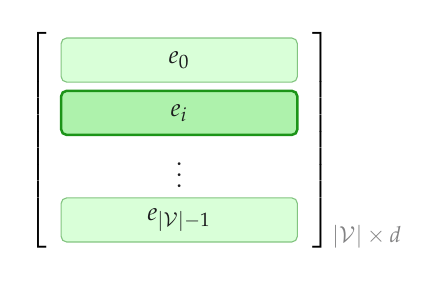
\begin{tikzpicture}
\matrix[matrix of nodes, left delimiter={[},right delimiter={]}, row sep=2.5pt, nodes={rowG}] (We) {
  $e_{0}$ \\ |[rowGhi]| $e_{i}$ \\ |[draw=none,fill=none]| $\vdots$ \\ $e_{|\mathcal{V}|-1}$ \\ };
\node[font=\footnotesize, softgray, anchor=west] at ([xshift=5pt,yshift=2mm]We.south east) {$|\mathcal{V}|\times d$};
\end{tikzpicture}
\figcap{\textbf{$W_{\text{embed}}$.} One row per vocabulary token; the lookup for token $i$ returns row $i$. Width $d$ = model dimension.}
\end{center}

That vector $e_i$ is everything the model knows about the token before it has seen any context, and that qualifier matters in two ways. First, the embedding is the same every time the token appears, no matter what surrounds it. The word \textit{bank} receives one fixed vector whether the sentence is about a river or a savings account, so $e_i$ can only capture a kind of blurred blend of its senses a token ever has. Sharpening that blur into a single intended sense is the job of attention, later, and is the reason the model needs context at all. Second, the embedding is blind to position. A token maps to the same vector whether it is the first word or the hundredth, because the lookup depends only on which token it is, never on where it sits. Before the representation can be useful, that missing piece, position, has to be supplied.

\subsubsection*{Positional Encoding}

Word order carries meaning, and a model that ignored it would miss much of what a sentence says. Reordering the words does change the input, since the rows end up in a different order, but it changes nothing else, as each word fetches the same vector wherever it sits. Two phrases with the same tokens in different orders therefore arrive as the same set of embeddings, merely rearranged, and the sole trace of order is the order of the rows. That trace goes unused, because attention inherently treats the rows as an unordered set, reading each token from its content and ignoring where it sits. Position must therefore be written into the vectors themselves, so the order-blind layers ahead can see it.

Positional encoding repairs this by giving each position its own signature. Position $i$ is assigned a vector $p_i \in \mathbb{R}^{1 \times d}$ that depends only on the slot, not on the word filling it, and this signature is combined with the token's embedding. How the signature is produced varies by model. It may be learned, as a separate table of vectors indexed by position, or computed from a fixed formula, as in the sinusoidal\footnote{As of 2026, many modern models take a different route. Rotary position embeddings (RoPE), for instance, inject position not by adding a vector here but by \emph{rotating} each token's query and key inside the attention computation, turning them by an angle that grows with the token's position (e.g., the tenth token's query is rotated twice as far as the fifth's, so tokens near the end of a long sequence arrive rotated furthest). The effect is that attention ends up encoding \emph{relative} distance rather than absolute slots. The principle is the same as in the additive scheme used here, that position must enter somewhere, even when the mechanism differs.} pattern of the original Transformer \citep{vaswani2017attention}. In these additive schemes the two pieces of information are simply summed,
\[
x_i = e_i + p_i \in \mathbb{R}^{1 \times d},
\]
so that a single vector now records both \textit{what} the token is, through $e_i$, and \textit{where} it sits, through $p_i$. 

Stacking the $n$ resulting vectors as rows gives the input matrix $X \in \mathbb{R}^{n \times d}$, with $X$ now carrying both meaning and order. This is the matrix that enters the first transformer block.

%==============================================================================
\newpage
\section{Layer Normalisation}
\label{sec:layernorm}
\heremap{ln}
%==============================================================================

Every transformer block applies layer normalisation, usually shortened to \textit{layer norm}, at two points: once before attention and once before the feedforward network\footnote{Normalising \textit{before} each sub-layer is called Pre-Norm. The original Transformer \citep{vaswani2017attention} normalised \textit{after} each sub-layer instead (Post-Norm), but most modern models use Pre-Norm because it trains more stably at depth.}. Its job is to keep the numbers flowing through the network at a steady, predictable scale. A token's vector is just a list of numbers, and every layer changes those numbers a little as the vector passes through. Across many layers these changes accumulate, and there is nothing in the design that keeps the numbers within any fixed range. They can grow much larger or shrink much smaller from one layer to the next, and that instability is a problem above all for \textit{training}. 

During training, a weight matrix is learned gradually, through many small corrections that nudge it towards detecting its feature a little better each time. The size of each correction tracks the size of the inputs it was computed from. If that scale lurches from layer to layer, the corrections lurch with it, too large at one moment and too small at the next, and learning becomes slow, unsteady, and can stall altogether. Layer norm removes the problem at its source by resetting each vector to a \textit{standard scale} before it reaches the next computation, so that the matrices that follow ($W_Q$, $W_K$, $W_V$, and the feedforward weights $W_1$, $W_2$) always meet inputs in a familiar range.

\subsubsection*{Normalisation or Standardisation?}

A quick word on terminology, because the two terms are easy to confuse and layer norm sits right on the seam between them. In statistics, \textit{standardisation} has a precise meaning: take a set of numbers, shift them so their average is zero, then divide by their standard deviation so that the spread becomes exactly one (e.g., z-score). \textit{Normalisation} is the looser, more general word for putting numbers onto a common, comparable scale by whatever means; min–max scaling, for instance, maps the smallest value to $0$ and the largest to $1$ via $(x-\min)/(\max-\min)$. The operation layer norm actually performs is, strictly speaking, standardisation. It computes a z-score for each token, across that token's features. But the technique is named for the broader goal it serves, which is to keep every token's vector on a predictable, common scale.

\subsubsection*{The Computation}

Layer norm works on one token at a time, using only that token's own numbers. Given token $i$'s embedding $\mathbf{x}_i \in \mathbb{R}^{1 \times d}$, it first finds the mean $\mu_i$ and standard deviation $\sigma_i$ of the $d$ values inside that single vector, then standardises them,
\[
\hat{\mathbf{x}}_i = \frac{\mathbf{x}_i - \mu_i}{\sqrt{\sigma_i^2 + \epsilon}}.
\]
The small constant $\epsilon$, around $10^{-5}$, sits inside the square root and guards against dividing by zero in the rare case that a token's values are all identical, which would otherwise make $\sigma_i^2$ vanish. Note that this is done \textit{independently} for each token, so one token's rescaling never depends on another's.

Standardising a vector might sound destructive. If we slide and squeeze its numbers, do we not also damage the meaning they carry? Section~2 gives us the vocabulary for a precise answer. Meaning, on the picture built there, lives in the \emph{direction} a vector points, not in its overall size, and standardisation barely touches direction. Dividing by the spread changes the vector's length alone. Subtracting the mean erases exactly one direction, the uniform one, along which every entry rises or falls by the same amount.

\subsubsection*{The Learned Adjustment}

Standardisation alone is a blunt reset. It forces every token to average exactly zero and spread exactly one, which is stable but rigid, since some axes may deserve more weight, or a different centre, than this one-size-fits-all standard permits. So layer norm follows the reset with a small learned adjustment,
\[
\mathbf{x}_{i,\text{norm}} = \gamma \odot \hat{\mathbf{x}}_i + \beta,
\]
where $\gamma$ rescales the standardised vector and $\beta$ shifts it. The parameters $\gamma, \beta \in \mathbb{R}^{d}$ act one axis at a time, with $\gamma_j$ setting the scale of axis $j$ and $\beta_j$ its centre, and they are shared across all tokens and learned alongside the rest of the network's weights.

What layer norm allows is thus a common footing. Standing in front of every major computation in the block, it ensures the attention and the feedforward network always read a vector on the same steady, learned scale. With the input now normalised, we can turn to the heart of the block, where attention projects each token into queries, keys, and values.

\newpage
\section{The Q, K, V Projections}
\heremap{qkv}
%==============================================================================

The heart of attention is three linear transformations applied to the same input. Each takes a token's representation and re-expresses it for a different purpose, and all three are exactly the kind of operation we studied in Section~2, a matrix multiplication, read here through the \meas{measurement}\footnote{Whenever attention or the feedforward network \emph{reads} from the residual stream, multiplying it by a weight matrix, the natural reading is measurement, the stream's content scored against learned directions. Whenever a sublayer \emph{writes} its result back to the stream, the natural reading is mixing, a blend of learned vectors added into the stream. Reading measures; writing mixes.} lens. Recall that each token's representation $x_i \in \mathbb{R}^{1 \times d}$ already encodes both what the token is and where it appears. The projection step asks three different sets of questions of that representation.

Let's take $Q$, the first of the three. The product $Q = X_{\text{norm}} W_Q$ multiplies each token's normalised embedding $x_{i,\text{norm}}$ by the matrix $W_Q \in \mathbb{R}^{d \times d_k}$, giving that token its query $q_i = x_{i,\text{norm}} W_Q$. Writing $W_Q$ as a collection of $d_k$ columns, each a $d$-dimensional vector, this projection is nothing more than $d_k$ dot products computed at once, one against each column.

\[
q_i = \begin{bmatrix} x_{i,\text{norm}} \cdot c_1 & x_{i,\text{norm}} \cdot c_2 & \cdots & x_{i,\text{norm}} \cdot c_{d_k} \end{bmatrix}_{1 \times d_k}
\]

\begin{center}
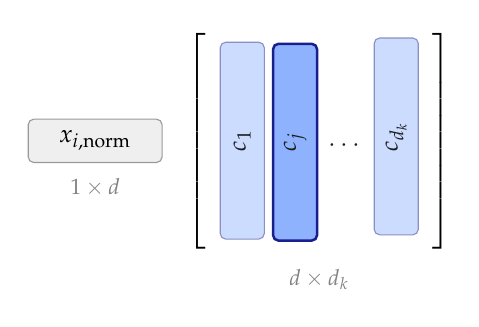
\begin{tikzpicture}
% x_{i,norm} row vector (neutral strip), to the LEFT of W_Q's columns
\node[draw=ink!45, fill=ink!7, rounded corners=2pt, minimum width=1.7cm, minimum height=0.55cm,
      font=\small, inner sep=1pt] (xr) {$x_{i,\text{norm}}$};
\node[font=\footnotesize, softgray, anchor=north] at ([yshift=-2pt]xr.south) {$1 \times d$};
\matrix[matrix of nodes, left delimiter={[},right delimiter={]}, column sep=2.5pt,
        ampersand replacement=\&, nodes={colB}, right=6mm of xr] (Wq) {
  \rotatebox{90}{$c_{1}$} \& |[colBhi]| \rotatebox{90}{$c_{j}$} \&
  |[draw=none,fill=none,minimum width=0.4cm]| $\cdots$ \& \rotatebox{90}{$c_{d_k}$} \\ };
\node[font=\footnotesize, softgray, anchor=north] at ([yshift=-2pt]Wq.south) {$d \times d_k$};
\end{tikzpicture}
\figcap{\textbf{$W_Q$} (and $W_K$, $W_V$ alike). Each column is one direction the token $x_{i,\text{norm}}$ (left) is scored against; $X_{\text{norm}}W_Q$ projects every token onto all $d_k$ of them at once. Recall that the machine learning community calls $W_Q$ a \textit{projection}, in the loose sense we met in Section~2, meaning any learned linear map that carries vectors from one space into another.}
\end{center}

Dotting $x_i$ against column $c_j$ asks how strongly the token exhibits the particular blend of features that $c_j$ weighs, and returns a single score. The $d_k$ columns ask $d_k$ such questions in parallel, so the output $q_i$ is a compact profile of the token, reading off how it scores on question~1, question~2, and so on up to question~$d_k$. 

These ``questions'' themselves are also learned. At the start of training the columns are random, asking arbitrary questions whose answers mean nothing, and training gradually reshapes them into questions worth asking, even though we usually cannot put a human name to what any single one detects. One might come to track a token's grammatical role, another its broad topic, but these are guesses\footnote{A research field, \emph{mechanistic interpretability}, is devoted to this problem, working to replace guesses about what a network's parts detect. A foundational work is the mathematical framework of transformer circuits~\citep{elhage2021mathematical}.} at an organisation the network arrives at on its own.

\begin{center}
\resizebox{7.5cm}{!}{%
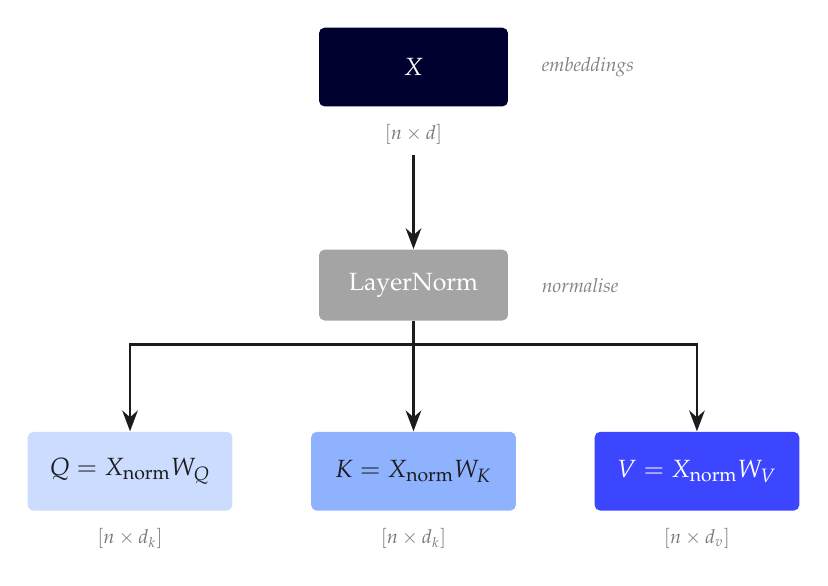
\begin{tikzpicture}[node distance=0.4cm and 0.7cm,
   mnode/.style={fbox, minimum width=2.4cm, minimum height=1.0cm},
   qkv/.style={fbox, minimum width=2.6cm, minimum height=1.0cm},
   normm/.style={fbox, minimum width=2.4cm, minimum height=0.9cm}]
  \node[mnode, sData] (X) {$X$};
  \node[sDim, below=0.10cm of X] (Xdim) {$[n \times d]$};
  \node[sLbl, right=0.3cm of X] {embeddings};
  \node[normm, sNorm, below=1.2cm of Xdim] (LN1) {LayerNorm};
  \node[sLbl, right=0.3cm of LN1] {normalise};
  \draw[sArrow] (Xdim.south) -- ++(0,-0.22) -- (LN1.north);
  \node[qkv, sBlueL, below=1.4cm of LN1, xshift=-3.6cm] (Q) {$Q = X_{\text{norm}}W_Q$};
  \node[sDim, below=0.10cm of Q] (Qdim) {$[n \times d_k]$};
  \node[qkv, sBlueM, below=1.4cm of LN1] (K) {$K = X_{\text{norm}}W_K$};
  \node[sDim, below=0.10cm of K] (Kdim) {$[n \times d_k]$};
  \node[qkv, sBlueB, below=1.4cm of LN1, xshift=3.6cm] (V) {$V = X_{\text{norm}}W_V$};
  \node[sDim, below=0.10cm of V] (Vdim) {$[n \times d_v]$};
  \coordinate (bp) at ($(LN1.south) + (0,-0.3)$);
  \draw[sArrow] (LN1.south) -- (bp) -| (Q.north);
  \draw[sArrow] (bp) -- (K.north);
  \draw[sArrow] (bp) -| (V.north);
\end{tikzpicture}}
\figcap{\textbf{The three projections.} The normalised representation is sent through three separate weight matrices, producing the query, key, and value profiles of every token.}
\end{center}

The same reading applies to the other two matrices. Each of $W_K$ and $W_V$ is likewise a stack of columns, and each column asks its own learned question of the same embedding $x_{i,\text{norm}}$. The essential picture is that one token representation is put through three different sets of questions at once, producing three different profiles of the same token, $q_i$, $k_i$, and $v_i$. All three descend from the very same row of $X$, the one vector carrying the token's identity and position. They differ only in which questions are asked.

\subsubsection*{A Note on the Names}

Nothing so far has explained the names. We have three sets of questions and three profiles of the same token; calling one a query, another a key, and the third a value has not yet been earned.

A common and useful picture compares attention to a lookup in a dictionary. A query is matched against a set of keys, and the value filed under the best-matching key is returned, except that here the match is ``soft'', meaning that every key's value contributes a little rather than one winning outright. It is a good first intuition, and we will recover it.

But we will not start from it, because starting there invites us to simply accept that one matrix \textit{is} the queries and another \textit{is} the keys, as though the names were assigned by decree. They are not. The roles are going to \textit{emerge} from the computation, and the names will turn out to fit for a precise reason, one that has nothing to do with the dictionary metaphor and everything to do with the arithmetic of the next two sections. So for now, treat the following as provisional labels rather than established facts,
\begin{itemize}
    \item $q_i = x_{i,\text{norm}} W_Q$, loosely, what token $i$ is looking for,
    \item $k_i = x_{i,\text{norm}} W_K$, loosely, what token $i$ offers to others,
    \item $v_i = x_{i,\text{norm}} W_V$, loosely, the content token $i$ contributes when attended to.
\end{itemize}

At this stage these are just three different linear maps of the same input, and nothing we have written so far forces them into these roles. Why a token's query should seek, and why its key should be the thing sought, all of this comes from where each matrix sits in the computation that follows.

%==============================================================================
\newpage
\section{Attention Scores}
\heremap{score,soft}
%==============================================================================

The previous section left us with three profiles of each token ($q_i$, $k_i$, and $v_i$) and an open question. We attached provisional names to them, but nothing yet justified those names. The three matrices are just three different linear maps. This section is where that changes. By the end of it the labels \textit{query} and \textit{key} will have earned themselves, and we will see what forces them apart. 

The full attention computation is
\[
\text{Attention}(Q,K,V) = \text{softmax}\!\left(\frac{QK^\top}{\sqrt{d_k}}\right) V,
\]
and we will take it in two stages: the scores $QK^\top$ in this section, and the retrieval by $V$ later. Notice first that the comparison itself does not care which token plays which role. Measuring how well a query matches a key is a dot product, and a dot product treats its two arguments alike. So nothing in the act of measuring one token against another favours the query side or the key side; whatever ends up distinguishing the two roles must come from elsewhere in the computation.

\subsubsection*{Attention Score Matrix}

Consider the product $QK^\top$. With $Q \in \mathbb{R}^{n \times d_k}$ and $K \in \mathbb{R}^{n \times d_k}$, transposing $K$ gives a $d_k \times n$ matrix, so the product is $n \times n$.

\begin{center}
\resizebox{\linewidth}{!}{%
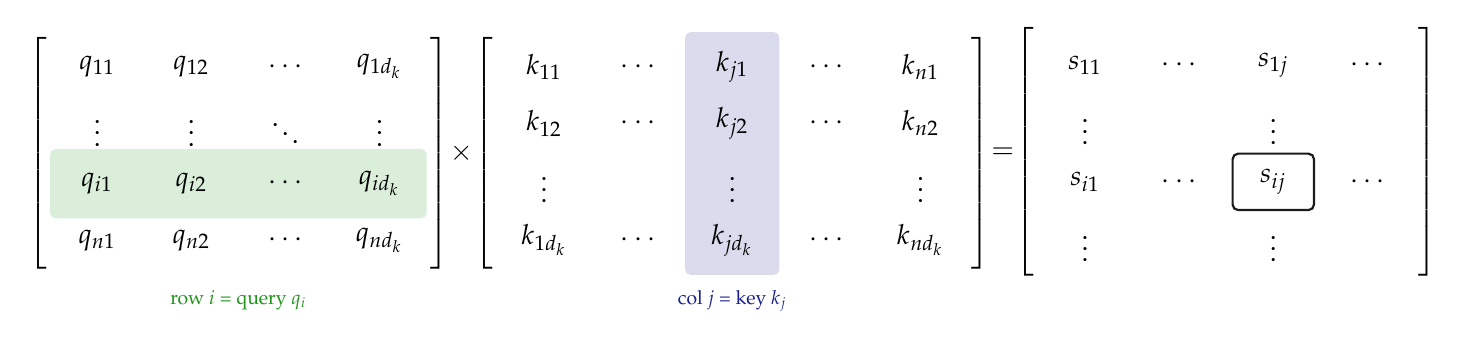
\begin{tikzpicture}[baseline]
  \matrix[matw] (Q) { q_{11} \& q_{12} \& \cdots \& q_{1d_k} \\
                      \vdots \& \vdots \& \ddots \& \vdots \\
                      q_{i1} \& q_{i2} \& \cdots \& q_{id_k} \\
                      q_{n1} \& q_{n2} \& \cdots \& q_{nd_k} \\ };
  \node[right=5pt of Q] (t) {$\times$};
  \matrix[matw, right=5pt of t] (K) { k_{11} \& \cdots \& k_{j1} \& \cdots \& k_{n1} \\
                      k_{12} \& \cdots \& k_{j2} \& \cdots \& k_{n2} \\
                      \vdots \& \& \vdots \& \& \vdots \\
                      k_{1d_k} \& \cdots \& k_{jd_k} \& \cdots \& k_{nd_k} \\ };
  \node[right=5pt of K] (e) {$=$};
  \matrix[matw, right=5pt of e] (S) { s_{11} \& \cdots \& s_{1j} \& \cdots \\
                      \vdots \& \& \vdots \& \\ s_{i1} \& \cdots \& s_{ij} \& \cdots \\
                      \vdots \& \& \vdots \& \\ };
  \begin{scope}[on background layer]
    \node[fill=mixink!16, rounded corners=2pt, fit=(Q-3-1)(Q-3-4)] {};
    \node[fill=measink!16, rounded corners=2pt, fit=(K-1-3)(K-4-3)] {};
  \end{scope}
  \node[draw=ink, line width=0.8pt, rounded corners=2pt, inner sep=1pt, fit=(S-3-3)] {};
  \node[below=2pt of Q.south, font=\scriptsize, mixink] {row $i$ = query $q_i$};
  \node[below=2pt of K.south, font=\scriptsize, measink] {col $j$ = key $k_j$};
\end{tikzpicture}}
\figcap{\textbf{The raw scores $QK^\top$.} The boxed entry $s_{ij}=q_i\cdot k_j$ is query~$i$ met with key~$j$. ($K^\top$ shown directly, so its columns are the keys; dividing by $\sqrt{d_k}$ gives the scaled score matrix $S$, keeping scores at a steady size so the softmax ahead stays soft.)}
\end{center}

Entry $(i,j)$ is the dot product $q_i \cdot k_j$. Read in the measurement language of Section~2, it scores how strongly position $i$'s query aligns with position $j$'s key --- a single number for how well what token $i$ is looking for matches what token $j$ offers. A large positive score means the match is strong; a score near zero means they are unrelated; a negative score means they actively pull apart.

\subsubsection*{Softmax Turns Scores into Attention}

Nothing so far has distinguished the query role from the key role. The rule filling each entry (i.e., dot a query against a key) draws no line between the two. What finally separates the roles is the next step, the softmax that turns these raw scores into attention.

% \footnote{Softmax exponentiates each score and then divides by the total, and the exponential grows very fast. Take three scores $2,\,1,\,0$: exponentiating gives about $7.4,\,2.7,\,1$, and dividing by their sum spreads the weight as roughly $0.67,\,0.24,\,0.09$ --- comfortably soft. Now multiply the same three scores by ten, to $20,\,10,\,0$: exponentiating gives about $4.9\times10^{8},\,2.2\times10^{4},\,1$, and the largest term now swamps the others, taking essentially all the weight while the rest round to zero. The larger the scores, the more sharply the biggest one dominates, until the softmax collapses onto a single position. Keeping the scores small keeps the weight spread out.}
% \footnote{The division by $\sqrt{d_k}$ is a scale correction, there to stop the scores growing with the head dimension, since feeding large numbers into a softmax makes it collapse onto a single position. Why $\sqrt{d_k}$ in particular, and not $d_k$? A dot product adds up $d_k$ separate pieces, some positive and some negative, and as they pile up they largely cancel out. A total built this way does not grow as fast as the number of pieces. It grows far more slowly, roughly like the \textit{square root} of that number. If $d_k$ is $100$, for instance, the total tends to land around $10$, not $100$. It is the same reason a hundred coin flips usually come out near fifty heads rather than ninety, since the heads and tails mostly offset and only a small swing is left over. A dot product over $d_k$ terms therefore has a typical size of about $\sqrt{d_k}$, and dividing by exactly that keeps it at a steady scale no matter how large $d_k$ grows.}

Softmax is applied \textit{one row at a time} to the scaled scores $S = QK^{\top}\!/\sqrt{d_k}$, turning each row into non-negative weights that sum to one,

\[
A_{ij} = \frac{\exp(S_{ij})}{\sum_{j'=1}^{n} \exp(S_{ij'})}.
\]

\textit{The decisive point is that softmax acts along rows, not columns}, and this treats the two directions of the matrix completely differently. Each row is forced into a probability distribution: a query must spend exactly one unit of attention, no more and no less, divided among the keys according to how well each matched. Whereas columns are bound by nothing. A key's column can sum to almost anything, depending on how many queries happened to want it. 

% \[
% \sum_{j=1}^{n} A_{ij} = 1 \qquad \text{whereas} \qquad \sum_{i=1}^{n} A_{ij} \neq 1 \; (\text{in general})
% \]

\begin{center}
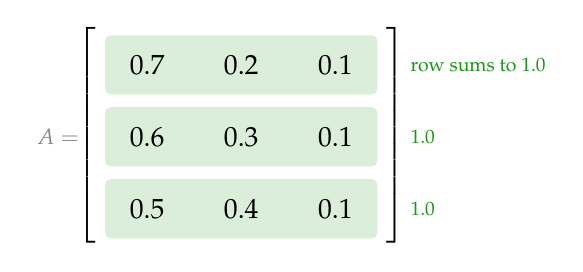
\begin{tikzpicture}[baseline]
\matrix[matw, row sep=8pt] (A) { 0.7 \& 0.2 \& 0.1 \\ 0.6 \& 0.3 \& 0.1 \\ 0.5 \& 0.4 \& 0.1 \\ };
\begin{scope}[on background layer]
  \foreach \r in {1,2,3} \node[fill=mixink!16, rounded corners=2pt, inner sep=1.5pt, fit=(A-\r-1)(A-\r-3)] {};
\end{scope}
\node[right=10pt of A-1-3, font=\scriptsize, mixink] {row sums to $1.0$};
\node[right=10pt of A-2-3, font=\scriptsize, mixink] {$1.0$};
\node[right=10pt of A-3-3, font=\scriptsize, mixink] {$1.0$};
\node[left=4pt of A, font=\footnotesize, softgray] {$A=$};
\end{tikzpicture}
\figcap{\textbf{Rows are probability distributions.} Each query spends exactly one unit of attention, divided among the keys --- so every row of $A$ sums to one.}
\end{center}

\begin{center}
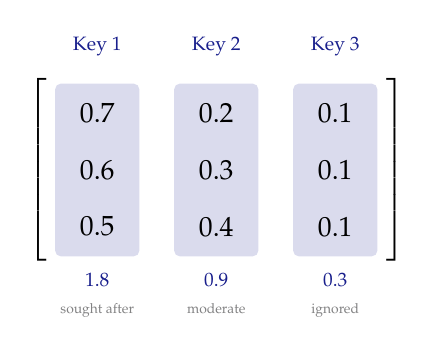
\begin{tikzpicture}[baseline]
\matrix[matw, column sep=16pt] (A) { 0.7 \& 0.2 \& 0.1 \\ 0.6 \& 0.3 \& 0.1 \\ 0.5 \& 0.4 \& 0.1 \\ };
\begin{scope}[on background layer]
  \foreach \c in {1,2,3} \node[fill=measink!16, rounded corners=2pt, inner sep=1.5pt, fit=(A-1-\c)(A-3-\c)] {};
\end{scope}
\node[above=8pt of A-1-1, font=\scriptsize, measink] {Key 1};
\node[above=8pt of A-1-2, font=\scriptsize, measink] {Key 2};
\node[above=8pt of A-1-3, font=\scriptsize, measink] {Key 3};
\node[below=4pt of A-3-1, font=\scriptsize\bfseries, measink] {$1.8$};
\node[below=4pt of A-3-2, font=\scriptsize\bfseries, measink] {$0.9$};
\node[below=4pt of A-3-3, font=\scriptsize\bfseries, measink] {$0.3$};
\node[below=15pt of A-3-1, font=\tiny, softgray] {sought after};
\node[below=15pt of A-3-2, font=\tiny, softgray] {moderate};
\node[below=15pt of A-3-3, font=\tiny, softgray] {ignored};
\end{tikzpicture}
\figcap{\textbf{Columns are under no constraint.} Column sums (how much total attention each key drew) are free: Key~1 pulls $1.8$, Key~3 only $0.3$, though every query divided its own unit fairly.}
\end{center}

This is the asymmetry the section was driving towards, and it gives queries and keys genuinely different natures. Read across a row, a query holds a fixed budget of one unit of attention and is guaranteed to spend all of it, so however the scores fall, every query comes away having gathered something. Read down a column, a key has no such guarantee. It is merely available to be matched, and whether it is attended to heavily, lightly, or not at all is decided entirely by how well it answers the needs of the queries around it.

Thus, \emph{a query behaves like a seeker that will always retrieve; a key behaves like a candidate competing to be retrieved}.

\subsubsection*{What This Means for Learning}

We can now say, at least in spirit, why $W_Q$ and $W_K$ end up doing different jobs even though they have the same shape and start from the same random initialisation. The two matrices sit in different positions in the computation, so they are shaped by different feedback. A query is always judged on what it manages to gather, so $W_Q$ is pushed to produce queries that align with the keys actually worth gathering. A key earns influence only when queries choose it, so $W_K$ is pushed to make tokens findable by the queries that should want them. Same arithmetic, opposite sides of it, and the pressure on each reflects the side it sits on. Nothing here was designed by hand. The structure creates the pressure, and training\footnote{During training, the model improves by nudging $W_Q$ and $W_K$ a little after each mistake (these nudges are what training calls \emph{gradients}). Picture the attention weights as a grid, one row per query and one column per key. The correction to a query is built from its own \textit{row}, that is, from how that single query spread its attention across the tokens. The correction to a key is built from its \textit{column}, gathering every query that did or did not attend to it. One matrix is therefore corrected a row at a time and the other a column at a time, so the two receive different feedback, and that is part of why they come to specialise. Working the corrections out in full is beyond our forward-pass scope.} does the rest.

The third matrix, $W_V$, sits outside all of this. It takes no part in the competition over who attends to whom --- it lives outside the softmax entirely --- and it learns something different: what a token should contribute once it has been attended to. We will see it work in Section~9. First, though, the mechanism as described lets every query reach every key, and for a model that generates text left to right that is too much freedom. The next section adds the one constraint that makes autoregressive generation possible, restricting each position to attend only to itself and the positions before it.

%==============================================================================
\newpage
\section{Causal (Autoregressive) Masking}
\heremap{mask}
%==============================================================================

The attention we have built earlier lets every query reach every key. A model that writes text one token at a time cannot be allowed that, so this section adds a single constraint, each position may attend only to itself and the positions before it, by ``hiding'' the future from every position even when the future happens to be present.

That ``hiding'' takes a single addition. Before the softmax, we add a mask $M$ to the scores, holding $0$ wherever a position is allowed to attend and $-\infty$ wherever it is not, so the attention computation reads
\[
\text{Attention}(Q, K, V) = \text{softmax}\!\left( \frac{QK^\top}{\sqrt{d_k}} + M \right) V.
\]

\begin{center}
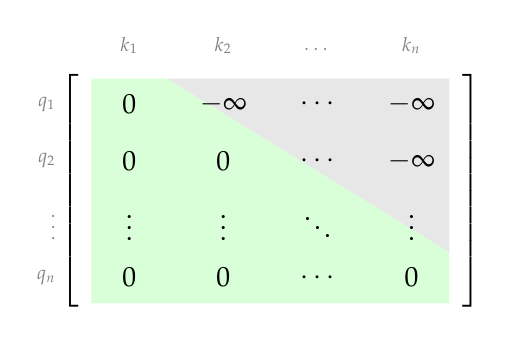
\begin{tikzpicture}[baseline]
  \matrix[matw] (M) {
    0 \& -\infty \& \cdots \& -\infty \\
    0 \& 0 \& \cdots \& -\infty \\
    \vdots \& \vdots \& \ddots \& \vdots \\
    0 \& 0 \& \cdots \& 0 \\ };
  \begin{scope}[on background layer]
    \fill[mixfill] (M-1-1.north west) -- (M-4-1.south west) -- (M-4-4.south east) -- (M-4-4.north east) -- (M-1-1.north east) -- cycle;
    \fill[greymask!22] (M-1-1.north east) -- (M-1-4.north east) -- (M-4-4.north east) -- cycle;
  \end{scope}
  \node[font=\scriptsize, softgray, anchor=south] at ([yshift=2pt]M.north-|M-1-1) {$k_1$};
  \node[font=\scriptsize, softgray, anchor=south] at ([yshift=2pt]M.north-|M-1-2) {$k_2$};
  \node[font=\scriptsize, softgray, anchor=south] at ([yshift=2pt]M.north-|M-1-3) {$\cdots$};
  \node[font=\scriptsize, softgray, anchor=south] at ([yshift=2pt]M.north-|M-1-4) {$k_n$};
  \node[font=\scriptsize, softgray, anchor=east] at ([xshift=-6pt]M.west|-M-1-1) {$q_1$};
  \node[font=\scriptsize, softgray, anchor=east] at ([xshift=-6pt]M.west|-M-2-1) {$q_2$};
  \node[font=\scriptsize, softgray, anchor=east] at ([xshift=-6pt]M.west|-M-3-1) {$\vdots$};
  \node[font=\scriptsize, softgray, anchor=east] at ([xshift=-6pt]M.west|-M-4-1) {$q_n$};
\end{tikzpicture}
\figcap{\textbf{The mask $M$.} Added to the scores just before the softmax: \mix{$0$} (lower triangle, $j\le i$) leaves a score untouched, while \textcolor{ink!55}{$-\infty$} (upper triangle, $j>i$) drives it to zero weight, since $e^{-\infty}=0$. The divide is the diagonal --- query~$i$ may attend to key~$j$ only when $j\le i$.}
\end{center}

Softmax exponentiates every score before normalising, and $\exp(-\infty) = 0$, so a masked position is driven to precisely zero weight. The allowed scores, with $0$ added, pass through unchanged.

The attention weights that come out are lower-triangular, empty above the diagonal.

\begin{center}
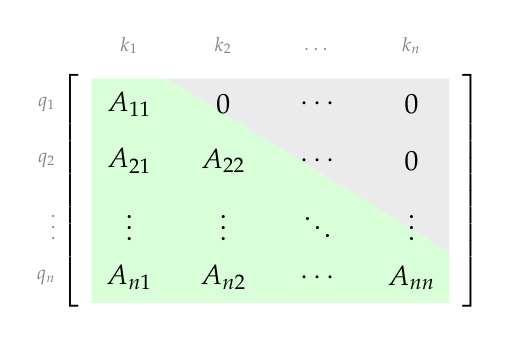
\begin{tikzpicture}[baseline]
  \matrix[matw] (Aw) {
    A_{11} \& 0 \& \cdots \& 0 \\
    A_{21} \& A_{22} \& \cdots \& 0 \\
    \vdots \& \vdots \& \ddots \& \vdots \\
    A_{n1} \& A_{n2} \& \cdots \& A_{nn} \\ };
  \begin{scope}[on background layer]
    \fill[mixfill] (Aw-1-1.north west) -- (Aw-4-1.south west) -- (Aw-4-4.south east) -- (Aw-4-4.north east) -- (Aw-1-1.north east) -- cycle;
    \fill[ink!9] (Aw-1-1.north east) -- (Aw-1-4.north east) -- (Aw-4-4.north east) -- cycle;
  \end{scope}
  \node[font=\scriptsize, softgray, anchor=south] at ([yshift=2pt]Aw.north-|Aw-1-1) {$k_1$};
  \node[font=\scriptsize, softgray, anchor=south] at ([yshift=2pt]Aw.north-|Aw-1-2) {$k_2$};
  \node[font=\scriptsize, softgray, anchor=south] at ([yshift=2pt]Aw.north-|Aw-1-3) {$\cdots$};
  \node[font=\scriptsize, softgray, anchor=south] at ([yshift=2pt]Aw.north-|Aw-1-4) {$k_n$};
  \node[font=\scriptsize, softgray, anchor=east] at ([xshift=-6pt]Aw.west|-Aw-1-1) {$q_1$};
  \node[font=\scriptsize, softgray, anchor=east] at ([xshift=-6pt]Aw.west|-Aw-2-1) {$q_2$};
  \node[font=\scriptsize, softgray, anchor=east] at ([xshift=-6pt]Aw.west|-Aw-3-1) {$\vdots$};
  \node[font=\scriptsize, softgray, anchor=east] at ([xshift=-6pt]Aw.west|-Aw-4-1) {$q_n$};
\end{tikzpicture}
\figcap{\textbf{Lower-triangular weights.} After the masked softmax every weight above the diagonal is zero (\textcolor{ink!55}{grey}); each query's surviving weights (\mix{green}) still sum to one. Row~$i$ spreads its attention over positions $1$ through $i$.}
\end{center}

The first position has no past, so it can only attend to itself. The second draws on positions one and two, the third on one through three, and so on. Every position now sees its own token and the ones before it, and nothing it could not yet know.

%==============================================================================
\newpage
\section{Value Retrieval}
\heremap{ret}
%==============================================================================

The attention weights tell each position \textit{where} to look, but not \textit{what} it finds there. The value vectors carry the what, and putting the two together is the step where information finally moves between positions. The head's output is a single multiplication,
\[
\text{head} = A(Q,K)\,V,
\]
which we will write simply as $AV$ from here on, the dependence on $Q$ and $K$ now understood.

% \begin{center}
% \begin{tikzpicture}[baseline]
%   \matrix[matw] (A) { a_{11} \& \cdots \& a_{1n} \\ \vdots \& \ddots \& \vdots \\ a_{n1} \& \cdots \& a_{nn} \\ };
%   \node[right=5pt of A] (t) {$\times$};
%   \matrix[matw, right=5pt of t] (V) { v_{11} \& \cdots \& v_{1d_v} \\ \vdots \& \ddots \& \vdots \\ v_{n1} \& \cdots \& v_{nd_v} \\ };
%   \node[right=5pt of V] (e) {$=$};
%   \matrix[matw, right=5pt of e] (O) { o_{11} \& \cdots \& o_{1d_v} \\ \vdots \& \ddots \& \vdots \\ o_{n1} \& \cdots \& o_{nd_v} \\ };
%   \begin{scope}[on background layer]
%     \node[fill=mixink!16, rounded corners=2pt, fit=(A-1-1)(A-1-3)] {};
%     \node[fill=measink!16, rounded corners=2pt, fit=(V-1-1)(V-3-1)] {};
%   \end{scope}
%   \node[draw=ink, line width=0.8pt, rounded corners=2pt, inner sep=1pt, fit=(O-1-1)] {};
%   \node[below=2pt of A.south, font=\scriptsize, mixink] {row $i$ = weights $a_i$};
%   \node[below=2pt of V.south, font=\scriptsize, measink] {col $j$ = value coord $j$};
% \end{tikzpicture}
% \figcap{\textbf{$\text{head}=AV$.} Output row $i$ is the value vectors blended by query $i$'s attention weights --- the mixing reading. The boxed entry is one coordinate of one output row.}
% \end{center}


\subsubsection*{Retrieval is Mixing}

This multiplication is the \textit{mixing} operation from Section~2, where the output row of a matrix product was a \textit{linear combination} of the rows of the right-hand matrix. Here the right-hand rows are the value vectors $v_1, \ldots, v_n$, each a learned projection of one token's representation.

\begin{center}
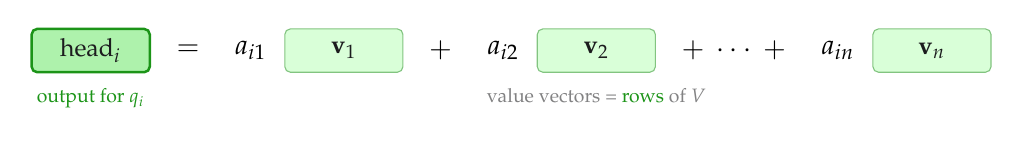
\begin{tikzpicture}[
   vstrip/.style={rounded corners=2pt, draw=mixink!55, fill=mixfill, text=ink, minimum width=1.5cm, minimum height=0.55cm, font=\small, inner sep=1pt},
   hstrip/.style={rounded corners=2pt, draw=mixink, line width=0.9pt, fill=mixfillb, text=ink, minimum width=1.5cm, minimum height=0.55cm, font=\small, inner sep=1pt}]
  \node[hstrip] (head) {$\text{head}_i$};
  \node[right=2mm of head] (eq) {$=$};
  \node[right=2mm of eq] (a1) {$a_{i1}$};
  \node[vstrip, right=1mm of a1] (v1) {$\mathbf{v}_1$};
  \node[right=2mm of v1] (p1) {$+$};
  \node[right=2mm of p1] (a2) {$a_{i2}$};
  \node[vstrip, right=1mm of a2] (v2) {$\mathbf{v}_2$};
  \node[right=2mm of v2] (p2) {$+\ \cdots\ +$};
  \node[right=2mm of p2] (an) {$a_{in}$};
  \node[vstrip, right=1mm of an] (vn) {$\mathbf{v}_n$};
  \node[font=\scriptsize, mixink, below=2pt of head] {output for $q_i$};
  \node[font=\scriptsize, softgray, below=2pt of v2] {value vectors = \mix{rows} of $V$};
\end{tikzpicture}
\figcap{\textbf{$\text{head}=AV$, read as mixing.} The output for query~$i$ is a weighted blend of the \emph{value vectors} $\mathbf{v}_1,\dots,\mathbf{v}_n$ --- the \mix{rows} of $V$ --- with weights $a_{i1},\dots,a_{in}$ taken from row~$i$ of $A$. The value vectors are a shared store; only the weights change from one query to the next, so every output is its own recipe over the same ingredients.}
\end{center}

Position $i$'s output is a blend of all the value vectors, with each $v_j$ poured in according to how much attention $i$ paid to position $j$. A position attended to heavily contributes most of its value, one barely attended contributes a trace, and one not attended at all contributes nothing.

\subsubsection*{What a Value Carries}

It remains to say what is actually being mixed. Like the query and key, the value is a learned view of the same token, computed by its own projection,
\[
V = X_{\text{norm}} W_V, \qquad v_i = x_{i,\text{norm}} W_V,
\]
where $W_V \in \mathbb{R}^{d \times d_v}$ is, like $W_Q$ and $W_K$, a stack of learned columns, each asking its own question of the embedding. The three projections differ only in what their questions are for. The columns of $W_Q$ shape what a token \textit{seeks}, those of $W_K$ shape what makes it \textit{findable}, and those of $W_V$ shape what it \textit{delivers} once found. As before, nothing fixes these questions in advance. The columns of $W_V$ begin random and are shaped by training to capture whatever a token can usefully pass on to the positions that attend to it. How a token is \textit{found} and what it \textit{transmits} can therefore be two different things; a noun located by a pronoun's search sends back its meaning, not its grammar, and nothing requires key and value to agree.
% \footnote{There is a tidy algebraic way to put the division. The score depends on $W_Q$ and $W_K$ only through their product, since $q_i \cdot k_j = x_{i,\text{norm}}\, (W_Q W_K^\top)\, x_{j,\text{norm}}^\top$, and what token $j$ contributes once attended to depends on $W_V$ and the later output matrix $W_O$ (Section~10) only through $W_V W_O$. Interpretability work, the study of what trained networks have actually learned, therefore treats an attention head as two separate low-rank maps (low-rank, meaning built from far fewer independent directions than $d$), a \emph{QK circuit} deciding where attention goes and an \emph{OV circuit} deciding what is written back once it does, with queries, keys, and values as intermediate products of this factorisation rather than its fundamental objects \citep{elhage2021mathematical}.}

This is the essence of attention. A token arrives at the layer describing mostly itself, and leaves describing itself in context, its representation updated by a blend of the values it attended to, each in proportion to the attention it drew. A token no longer merely carries its own meaning forward through the network; it absorbs context from the tokens around it, and what it absorbs reshapes what it represents.

That completes a single attention head. Everything it gathers, though, comes back as one blend under one set of proportions, and the next section asks what a layer gains by running several heads at once.

%==============================================================================
\newpage
\section{Multi-Head Attention}
\heremap{heads}
%==============================================================================

Everything so far has described \textit{single-head} attention, one set of projections $W_Q$, $W_K$, $W_V$, producing one attention pattern and one output. Often, in practice, transformers run several such mechanisms side by side, each with its own projections, and this section explains why that helps and how the parallel outputs are recombined.

\subsubsection*{Splitting Attention into Heads}

A single head can already look in several places at once. Its weights are a distribution, free to spread over a subject, a referent, and a topic alike. What it cannot do is keep those looks apart. The weights sum to one, so every need competes for the same budget, and everything retrieved comes back as one blend, gathered for different reasons yet averaged under the same proportions \citep{vaswani2017attention}. 

Multi-head attention pulls them apart. It runs $h$ smaller attentions, the \textit{heads}, each with its own budget, its own blend, and its own reason for looking. The model is given $h$ separate sets of projections, one per head, with head $i$ holding
\[
W_Q^{(i)}, W_K^{(i)} \in \mathbb{R}^{d \times d_k}, \qquad W_V^{(i)} \in \mathbb{R}^{d \times d_v}, \qquad \text{typically } d_k = d_v = d/h,
\]
and each head runs the entire attention mechanism of the previous sections --- scores, masking, softmax, and retrieval alike --- inside its own slice of the dimensions,
\[
\text{head}_i = \text{softmax}\!\left( \frac{Q_i K_i^\top}{\sqrt{d_k}} + M \right) V_i \in \mathbb{R}^{n \times d_v}
\]
\[
\qquad Q_i = X_{\text{norm}} W_Q^{(i)}, \quad K_i = X_{\text{norm}} W_K^{(i)}, \quad V_i = X_{\text{norm}} W_V^{(i)}
\]

What the split buys is $h$ separate budgets. Each head normalises its own scores,
so a token now spends one unit of attention \emph{per head} rather than one in
total, and the same pair of tokens draws $h$ weights instead of one. In practice, the per-head matrices are stacked side by side into one wide array, $W_Q = [\,W_Q^{(1)} \cdots W_Q^{(h)}\,] \in \mathbb{R}^{d \times d}$, and a single multiplication $X_{\text{norm}} W_Q$ produces every head's queries at once, with $K$ and $V$ handled likewise. The first $d_k$ columns of $X_{\text{norm}} W_Q$ are exactly $Q_1$, the next $d_k$ exactly $Q_2$, and the wide array is $h$ independent projections stored together.

What each head comes to specialise in is left to training. Every head's projections begin random, exactly as in the single-head case, and are shaped by the data, so one head may drift towards grammatical agreement, another towards meaning, another towards position. Figure~3 shows the full computation for $h = 4$: the input $X$ fans out into four parallel streams, each computing its own queries, keys, values, attention pattern, and retrieval, after which the four outputs are concatenated and passed through a final projection, the step we turn to next.

% What gives a head its own reason for looking? Only its columns. $W_Q^{(i)}$ has $d_k$ of them, each a learned direction, each a question. No other head owns those columns, and $K_i$ and $V_i$ have columns of their own in the same way. 


% Are the $h$ heads genuinely independent? The implementation invites doubt, since they are not computed separately at all. The per-head matrices are stacked side by side into one wide array, $W_Q = [\,W_Q^{(1)} \cdots W_Q^{(h)}\,] \in \mathbb{R}^{d \times d}$, and a single multiplication $X_{\text{norm}} W_Q$ produces every head's queries at once, with $K$ and $V$ handled likewise. Nothing is blended even so. A matrix product builds one output column at a time, each from its own column of $W_Q$ and no other, so no head's answers ever draw on another head's questions. The first $d_k$ columns of $X_{\text{norm}} W_Q$ are exactly $Q_1$, the next $d_k$ exactly $Q_2$, and the wide array is $h$ independent projections stored together for speed. Separate questions, though, only supply the raw material. What makes the heads genuinely many is where the softmax is applied. At full width it would score each token's whole profile of $d$ answers against every other token's, giving each pair one number and each query one ranking, which is single-head attention by another name. Applied block by block, to each head's own $Q_i K_i^\top$, it compares $Q_i$ against $K_i$ and nothing else, so the same pair of tokens receives $h$ numbers, one per set of questions. Two tokens may score high in one head and low in another, agreeing on what head~1 asked and differing on what head~2 asked. Each score is then normalised on its own, so each head spends its own budget and retrieves its own blend, the heads coming together only afterwards.

% \newpage
%=====================================================================
% Figure 3 : Multi-Head Attention
%=====================================================================
\begin{center}
\resizebox{0.86\textwidth}{!}{%
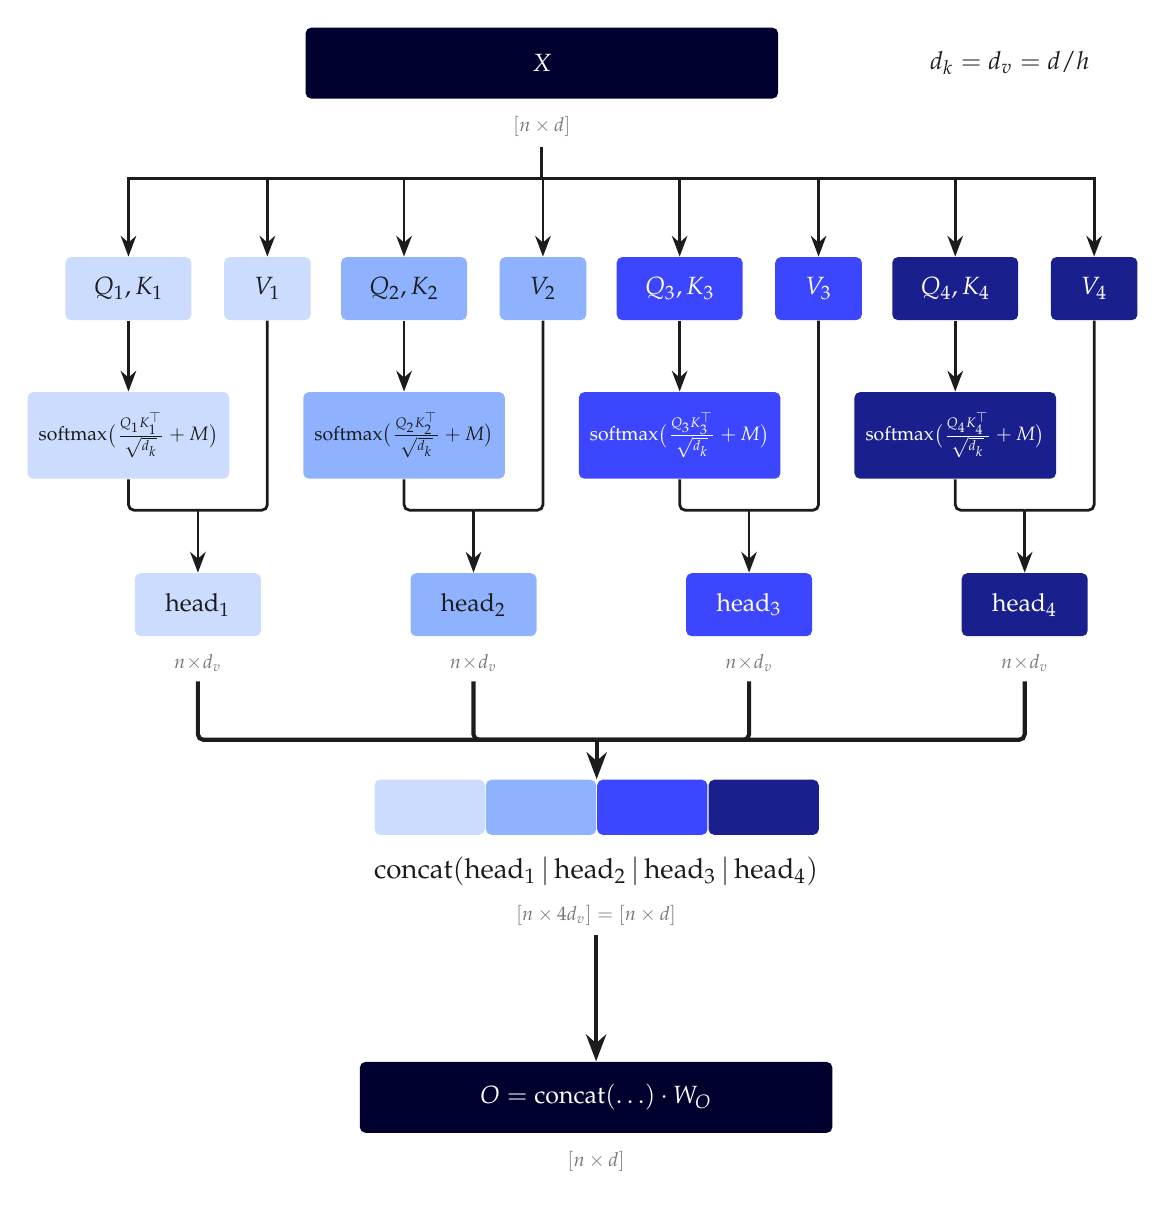
\begin{tikzpicture}[node distance=0.6cm,
   fullm/.style={fbox, minimum width=6.0cm, minimum height=0.9cm},
   qkb/.style={fbox, minimum width=1.6cm, minimum height=0.8cm},
   vb/.style={fbox, minimum width=1.1cm, minimum height=0.8cm},
   attnb/.style={fbox, rounded corners=3pt, minimum width=2.0cm, minimum height=1.1cm},
   headmm/.style={fbox, minimum width=1.6cm, minimum height=0.8cm},
   cseg/.style={fbox, minimum width=1.4cm, minimum height=0.7cm}]
 
  \node[fullm, sData] (X) {$X$};
  \node[sDim, below=0.1cm of X] (Xdim) {$[n \times d]$};
 
  \def\hsp{3.5cm}\def\qg{0.4cm}
 
  % HEAD 1
  \node[qkb, sH1, below=2.0cm of X, xshift=-1.5*\hsp] (QK1) {$Q_1, K_1$};
  \node[vb, sH1, right=\qg of QK1] (V1) {$V_1$};
  \node[attnb, sH1, below=0.9cm of QK1] (attn1) {\scriptsize $\text{softmax}\big(\frac{Q_1 K_1^\top}{\sqrt{d_k}} + M\big)$};
  \coordinate (mid1) at ($(QK1.south)!0.5!(V1.south)$);
  \node[headmm, sH1, below=3.2cm of mid1] (head1) {$\text{head}_1$};
  \node[sDim, below=0.1cm of head1] (head1dim) {\scriptsize$n \!\times\! d_v$};
  \draw[sArrow] (QK1.south) -- (attn1.north);
  \coordinate (conv1) at ($(attn1.south)!0.5!(V1.south) + (0,-1.4)$);
  \draw[sLine, rounded corners=2pt] (attn1.south) |- (conv1);
  \draw[sLine, rounded corners=2pt] (V1.south) |- (conv1);
  \draw[sArrow] (conv1) -- (head1.north);
 
  % HEAD 2
  \node[qkb, sH2, below=2.0cm of X, xshift=-0.5*\hsp] (QK2) {$Q_2, K_2$};
  \node[vb, sH2, right=\qg of QK2] (V2) {$V_2$};
  \node[attnb, sH2, below=0.9cm of QK2] (attn2) {\scriptsize $\text{softmax}\big(\frac{Q_2 K_2^\top}{\sqrt{d_k}} + M\big)$};
  \coordinate (mid2) at ($(QK2.south)!0.5!(V2.south)$);
  \node[headmm, sH2, below=3.2cm of mid2] (head2) {$\text{head}_2$};
  \node[sDim, below=0.1cm of head2] (head2dim) {\scriptsize$n \!\times\! d_v$};
  \draw[sArrow] (QK2.south) -- (attn2.north);
  \coordinate (conv2) at ($(attn2.south)!0.5!(V2.south) + (0,-1.4)$);
  \draw[sLine, rounded corners=2pt] (attn2.south) |- (conv2);
  \draw[sLine, rounded corners=2pt] (V2.south) |- (conv2);
  \draw[sArrow] (conv2) -- (head2.north);
 
  % HEAD 3
  \node[qkb, sH3, below=2.0cm of X, xshift=0.5*\hsp] (QK3) {$Q_3, K_3$};
  \node[vb, sH3, right=\qg of QK3] (V3) {$V_3$};
  \node[attnb, sH3, below=0.9cm of QK3] (attn3) {\scriptsize $\text{softmax}\big(\frac{Q_3 K_3^\top}{\sqrt{d_k}} + M\big)$};
  \coordinate (mid3) at ($(QK3.south)!0.5!(V3.south)$);
  \node[headmm, sH3, below=3.2cm of mid3] (head3) {$\text{head}_3$};
  \node[sDim, below=0.1cm of head3] (head3dim) {\scriptsize$n \!\times\! d_v$};
  \draw[sArrow] (QK3.south) -- (attn3.north);
  \coordinate (conv3) at ($(attn3.south)!0.5!(V3.south) + (0,-1.4)$);
  \draw[sLine, rounded corners=2pt] (attn3.south) |- (conv3);
  \draw[sLine, rounded corners=2pt] (V3.south) |- (conv3);
  \draw[sArrow] (conv3) -- (head3.north);
 
  % HEAD 4
  \node[qkb, sH4, below=2.0cm of X, xshift=1.5*\hsp] (QK4) {$Q_4, K_4$};
  \node[vb, sH4, right=\qg of QK4] (V4) {$V_4$};
  \node[attnb, sH4, below=0.9cm of QK4] (attn4) {\scriptsize $\text{softmax}\big(\frac{Q_4 K_4^\top}{\sqrt{d_k}} + M\big)$};
  \coordinate (mid4) at ($(QK4.south)!0.5!(V4.south)$);
  \node[headmm, sH4, below=3.2cm of mid4] (head4) {$\text{head}_4$};
  \node[sDim, below=0.1cm of head4] (head4dim) {\scriptsize$n \!\times\! d_v$};
  \draw[sArrow] (QK4.south) -- (attn4.north);
  \coordinate (conv4) at ($(attn4.south)!0.5!(V4.south) + (0,-1.4)$);
  \draw[sLine, rounded corners=2pt] (attn4.south) |- (conv4);
  \draw[sLine, rounded corners=2pt] (V4.south) |- (conv4);
  \draw[sArrow] (conv4) -- (head4.north);
 
  % branch from X
  \coordinate (bt) at ($(Xdim.south) + (0,-0.4)$);
  \draw[sArrow] (Xdim.south) -- (bt) -| (QK1.north);
  \draw[sArrow] (bt) -| (V1.north);
  \draw[sArrow] (bt) -| (QK2.north);
  \draw[sArrow] (bt) -| (V2.north);
  \draw[sArrow] (bt) -| (QK3.north);
  \draw[sArrow] (bt) -| (V3.north);
  \draw[sArrow] (bt) -| (QK4.north);
  \draw[sArrow] (bt) -| (V4.north);
 
  % concatenation
  \coordinate (cc) at ($(head1dim.south)!0.5!(head4dim.south) + (0,-1.6)$);
  \node[cseg, sH1, anchor=east] (c1) at ($(cc) + (-1.6,0)$) {};
  \node[cseg, sH2, anchor=west] (c2) at (c1.east) {};
  \node[cseg, sH3, anchor=west] (c3) at (c2.east) {};
  \node[cseg, sH4, anchor=west] (c4) at (c3.east) {};
 
  \coordinate (bb) at ($(c2.north)!0.5!(c3.north) + (0,0.5)$);
  \draw[sConcatLine, rounded corners=2pt] (head1dim.south) |- (bb);
  \draw[sConcatLine, rounded corners=2pt] (head2dim.south) |- (bb);
  \draw[sConcatLine, rounded corners=2pt] (head3dim.south) |- (bb);
  \draw[sConcatLine, rounded corners=2pt] (head4dim.south) |- (bb);
  \draw[sConcat] (bb) -- ($(c2.north)!0.5!(c3.north)$);
 
  \node[below=0.15cm of c2, xshift=0.7cm, text=ink] (clabel)
     {$\text{concat}(\text{head}_1 \,|\, \text{head}_2 \,|\, \text{head}_3 \,|\, \text{head}_4)$};
  \node[sDim, below=0.0cm of clabel] (cdim) {$[n \times 4d_v] = [n \times d]$};
 
  \node[fullm, sData, below=1.6cm of cdim] (O) {$O = \text{concat}(\ldots) \cdot W_O$};
  \node[sDim, below=0.1cm of O] {$[n \times d]$};
  \draw[sConcat] (cdim.south) -- ++(0,-0.35) -- (O.north);
 
  \node[anchor=west, font=\small, text=ink] at ($(X.east) + (1.8,0)$) {$d_k = d_v = d/h$};
\end{tikzpicture}}
\figcap{\textbf{Figure 3:} Multi-Head Attention}
\end{center}

\subsubsection*{Writing the Heads Back}

Each head returns an $n \times d_v$ matrix. Setting the $h$ of them side by side gives
\[
\text{concat}(\text{head}_1, \ldots, \text{head}_h) \in \mathbb{R}^{n \times h d_v} = \mathbb{R}^{n \times d},
\]
which lands back at width $d$ because $h d_v = d$. A final matrix $W_O \in \mathbb{R}^{d \times d}$ turns that into the layer's output, and we will use the \emph{mixing} reading. Read $W_O$ by its rows, where row~$r$ is a vector $\mathbf{w}_r$ of $d$ numbers, and a vector of $d$ numbers is a direction in the residual stream itself, so every row of $W_O$ already lives in the space the layer must write to. Write $\mathbf{h}_t$ for row~$t$ of the concatenation above, one vector of $d$ numbers.

\begin{center}
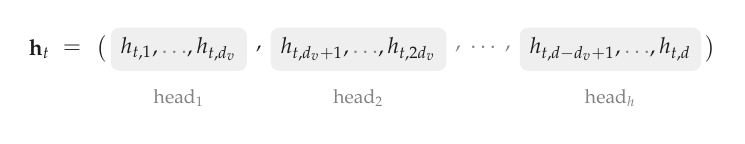
\begin{tikzpicture}[
  amt/.style={font=\footnotesize, text=ink, inner sep=0.4pt},
  dts/.style={font=\footnotesize, text=softgray, inner sep=0.4pt},
  sgn/.style={font=\footnotesize, text=ink, inner sep=0.4pt},
  hd/.style={font=\scriptsize, text=softgray}]

  \node[amt] (lhs) {$\mathbf{h}_t$};
  \node[sgn, right=1.2mm of lhs] (eq) {$=$};
  \node[sgn, right=1.4mm of eq]  (lp) {$\big($};

  % ---------------- one node per head's block ----------------
  \node[amt, right=1.4mm of lp] (g1)
        {$h_{t,1}, \textcolor{softgray}{\ldots}, h_{t,d_v}$};
  \node[sgn, right=2.0mm of g1] (s1) {$,$};
  \node[amt, right=2.0mm of s1] (g2)
        {$h_{t,d_v+1}, \textcolor{softgray}{\ldots}, h_{t,2d_v}$};
  \node[dts, right=2.0mm of g2] (s2) {$,\ \ldots\ ,$};
  \node[amt, right=2.0mm of s2] (g3)
        {$h_{t,d-d_v+1}, \textcolor{softgray}{\ldots}, h_{t,d}$};

  \node[sgn, right=1.4mm of g3] (rp) {$\big)$};

  % ---------------- one grey block per head ----------------
  \begin{scope}[on background layer]
    \node[rounded corners=3pt, fill=ink!7, inner xsep=3pt, inner ysep=3pt,
          fit=(g1)] (G1) {};
    \node[rounded corners=3pt, fill=ink!7, inner xsep=3pt, inner ysep=3pt,
          fit=(g2)] (G2) {};
    \node[rounded corners=3pt, fill=ink!7, inner xsep=3pt, inner ysep=3pt,
          fit=(g3)] (G3) {};
  \end{scope}

  \node[hd, below=1.0mm of G1] {$\text{head}_1$};
  \node[hd, below=1.0mm of G2] {$\text{head}_2$};
  \node[hd, below=1.0mm of G3] {$\text{head}_h$};

\end{tikzpicture}
\end{center}
\vspace{-0.7em}

\noindent Its entry $h_{t,r}$ says how much of direction $\mathbf{w}_r$ to write. Position $t$'s output is their blend,
\[
\mathbf{o}_t \;=\; \sum_{r=1}^{d} h_{t,r}\, \mathbf{w}_r \;\in\; \mathbb{R}^{1 \times d},
\]
a single vector in the stream's own coordinates, and $O$, the $n$ such rows stacked, is the full output of multi-head attention, ready to be added back.

\begin{center}
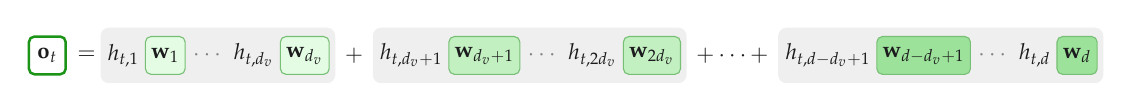
\begin{tikzpicture}[
  ostrip/.style={rounded corners=2pt, draw=mixink, line width=0.9pt, fill=white,
                 text=ink, minimum height=0.48cm, font=\footnotesize, inner xsep=3pt,
                 inner ysep=1.5pt},
  wstrip/.style={rounded corners=2pt, draw=mixink!60, text=ink, minimum height=0.48cm,
                 font=\footnotesize, inner xsep=2pt, inner ysep=1.5pt},
  amt/.style={font=\footnotesize, text=ink, inner sep=0.4pt},
  dts/.style={font=\footnotesize, text=softgray, inner sep=0.4pt},
  sgn/.style={font=\footnotesize, text=ink, inner sep=0.4pt}]

  \node[ostrip] (o) {$\mathbf{o}_t$};
  \node[sgn, right=1.1mm of o] (e) {$=$};

  % ---------------- head 1 ----------------
  \node[amt,    right=1.1mm of e]  (a1) {$h_{t,1}$};
  \node[wstrip, fill=hA, right=0.5mm of a1] (u1) {$\mathbf{w}_{1}$};
  \node[dts,    right=0.7mm of u1] (d1) {$\cdots$};
  \node[amt,    right=0.7mm of d1] (b1) {$h_{t,d_v}$};
  \node[wstrip, fill=hA, right=0.5mm of b1] (v1) {$\mathbf{w}_{d_v}$};

  % ---------------- head 2 ----------------
  \node[sgn,    right=1.7mm of v1] (p1) {$+$};
  \node[amt,    right=1.7mm of p1] (a2) {$h_{t,d_v+1}$};
  \node[wstrip, fill=hB, right=0.5mm of a2] (u2) {$\mathbf{w}_{d_v+1}$};
  \node[dts,    right=0.7mm of u2] (d2) {$\cdots$};
  \node[amt,    right=0.7mm of d2] (b2) {$h_{t,2d_v}$};
  \node[wstrip, fill=hB, right=0.5mm of b2] (v2) {$\mathbf{w}_{2d_v}$};

  % ---------------- head h ----------------
  \node[sgn,    right=1.7mm of v2] (p2) {$+\cdots+$};
  \node[amt,    right=1.7mm of p2] (a3) {$h_{t,d-d_v+1}$};
  \node[wstrip, fill=hC, right=0.5mm of a3] (u3) {$\mathbf{w}_{d-d_v+1}$};
  \node[dts,    right=0.7mm of u3] (d3) {$\cdots$};
  \node[amt,    right=0.7mm of d3] (b3) {$h_{t,d}$};
  \node[wstrip, fill=hC, right=0.5mm of b3] (v3) {$\mathbf{w}_{d}$};

  % ---------------- one band per head ----------------
  \begin{scope}[on background layer]
    \node[rounded corners=3pt, fill=ink!7, inner xsep=2pt, inner ysep=3pt,
          fit=(a1)(v1)] (B1) {};
    \node[rounded corners=3pt, fill=ink!7, inner xsep=2pt, inner ysep=3pt,
          fit=(a2)(v2)] (B2) {};
    \node[rounded corners=3pt, fill=ink!7, inner xsep=2pt, inner ysep=3pt,
          fit=(a3)(v3)] (B3) {};
  \end{scope}

\end{tikzpicture}
\figcap{\textbf{$\mathbf{o}_t = \mathbf{h}_t W_O$, read as mixing.} Every $\mathbf{w}_r$ is a \mix{row} of $W_O$, a direction in the $d$-dimensional stream, and the amount $h_{t,r}$ beside it says how much of that direction position~$t$ writes. The $d$ rows come in $h$ groups of $d_v$, one group per head, and a group spans the subspace that head writes into. Within a group the three dots stand for the $d_v - 2$ terms not shown, all of them added.}
\end{center}

% \subsubsection*{Do the Heads Really Get Used?}

% It is fair to ask whether a trained model exploits all this capacity or leaves heads idle. \citet{michel2019sixteen} probed this in two ways, working with the translation and inference models standard at the time rather than modern decoder-only LLMs. The first switches off individual heads within a single layer, leaving the rest of the model intact, and measures the damage, a technique called \textit{ablation}. In their setting many heads turned out to be removable with little loss, and some layers kept working even when stripped most of the way down towards a single head, despite having been trained with twelve or sixteen, though a subset of heads proved important and could not be removed cheaply.

% The second experiment was more global. Rather than work one layer at a time, it scored every head in the whole model by importance, estimated from how much the loss worsens when that head alone is switched off, and then \textit{pruned} them in order, removing the least important first. A sizeable fraction of heads could be discarded this way before accuracy fell off sharply. The two experiments differ in scope, one asking how much a single layer can spare and the other how much the model as a whole can spare, but they point the same way.

% These results come from particular architectures and tasks, so the exact numbers should not be read as universal, and whether they carry over cleanly to today's large autoregressive models is a reasonable question rather than a settled fact. The qualitative lesson is the durable part, and it is not that the extra heads are wasted. During training the many heads let the model explore a wide range of ways for tokens to relate, and the redundancy left over afterwards looks less like idle capacity than like robustness, a network that keeps functioning when a few of its parts are disturbed.

\subsubsection*{The Residual Connection}

Attention's output is added back to the same representation it was computed from, through a residual\footnote{The name is inherited from residual networks \citep{he2016deep}, where the input is carried forward unchanged and a sublayer needs to learn only the \emph{residual}, the difference between the input and the desired output. This running representation is often called the \textit{residual stream}. Each sublayer reads from it and adds its contribution back, so the stream accumulates the embedding, then attention's context, then the feedforward network's processing, and so on through the layers.} connection,
\[
X' = X + O,
\]
so that $X'$ now holds two things at once:
\begin{itemize}
    \item the original token embedding, preserved untouched through the addition, and
    \item the context gathered from other positions, added on top by attention.
\end{itemize}
Nothing has been overwritten. Attention only \textit{adds} to what was already there, which is also what lets these blocks be stacked to great depth. Because each sublayer writes its result onto a running representation rather than replacing it, it only has to learn a small correction to what the previous layers built, and the addition gives gradients a clean path back through the network during training.

This is also the limit of what attention can do. Although the attention weights are themselves produced nonlinearly (by the softmax), the step that uses them is linear. Given the weights, each position's output is a plain weighted average of value vectors already present, so attention can only ever return a linear mixture of its inputs, never a nonlinear transformation of their content. It can route information between positions and average it together, but the result is always built from the value vectors it started with, never a genuinely new quantity computed from them. This given-the-weights linearity is a workhorse of the interpretability literature \citep{elhage2021mathematical}. That is the job of the next component, the feedforward network, which takes the context attention has assembled at each position and actually processes it.

%==============================================================================
\newpage
\section{The Feedforward Network}
\heremap{ffn}
%==============================================================================

Multi-head attention left each position holding the context it had gathered from the rest of the sequence, recombined across heads and added back into its representation. But attention only ever \textit{moved} information between positions; it never transformed the content it carried. That is the feedforward network's job. Attention \textit{moves} information between positions, the feedforward network \textit{processes} it.

Once attention has gathered context from other tokens into each position, the feedforward network --- a small two-layer network --- works on each position on its own, putting every position through the very same transformation. This is its defining contrast with attention, which existed to let positions communicate. Attention mixes across tokens, the feedforward network thinks about each token in isolation.

Loosely speaking, the network reads then writes, and it does so through a shape of expand, process, contract. Each position's $d$-dimensional vector is first widened to a much larger $d_{\text{ff}}$ dimensions, typically four times $d$, then passed through a nonlinearity, then squeezed back down to $d$. The first matrix ($W_1$) scores the incoming vector against $d_{\text{ff}}$ learned directions at once (measurement), so the widening is really a bank of detectors, each asking whether some pattern is present and reporting how strongly. The nonlinearity then keeps the patterns that fired and suppresses the rest, and the second matrix ($W_2$) \textit{mixes} those surviving signals back down into a single $d$-dimensional vector, assembled as a recipe over learned components.

\subsubsection*{The Architecture}

As in the attention sublayer, the input is first passed through LayerNorm (Pre-Norm), stabilising its scale so the patterns $W_1$ looks for stay reliable from layer to layer (Section~5). Following the notation of Figure~2b, we write $X'$ for the post-attention representation entering this sublayer and $X'_{\text{norm}} = \text{LayerNorm}(X')$ for its normalised form. 

The network applies two linear maps with a nonlinearity, ReLU\footnote{We use ReLU throughout for simplicity, following the original Transformer \citep{vaswani2017attention}. Many modern LLMs use alternatives, such as the smoother GELU or gated units like SwiGLU and GeGLU. These can improve performance, but the expand, process, contract role of the sublayer remains the same. We also drop the bias terms throughout this section for simplicity, since they add nothing to the measurement-and-mixing reading that follows. A reader who prefers the fuller form can restore them, writing each linear map as $XW + b$ in place of $XW$.}, between them,
\[
\text{FFN}(X'_{\text{norm}}) = \text{ReLU}(X'_{\text{norm}} W_1)\, W_2,
\]
where $X'_{\text{norm}} \in \mathbb{R}^{n \times d}$ is the normalised post-attention representation, $W_1 \in \mathbb{R}^{d \times d_{\text{ff}}}$ does the widening, and $W_2 \in \mathbb{R}^{d_{\text{ff}} \times d}$ the squeezing back.

\subsubsection*{The First Layer Measures}

This is the measurement reading of Section~2. Each column of $W_1$ is a learned question, a $d$-dimensional pattern, and dotting a position's vector against it scores how strongly that pattern is present,
\[
(X'_{\text{norm}} W_1)_{ij} = x'_{i,\text{norm}} \cdot c_j,
\]
with $c_j$ the $j$-th column. Across all $d_{\text{ff}}$ columns, every position receives $d_{\text{ff}}$ scores, one per pattern. ReLU then zeroes the negatives, keeping a score only where the position's vector aligned positively with the column,
\[
H = \text{ReLU}(X'_{\text{norm}} W_1) \in \mathbb{R}^{n \times d_{\text{ff}}}.
\]

The result $H$ is best pictured as an on/off pattern. For each token, every one of the $d_{\text{ff}}$ entries is either zero, where the pattern was absent, or positive, where it fired, marking which patterns that token triggered (and, in the size of each nonzero entry, how strongly). Which entries are active varies from token to token, and that input-dependent pattern of who-fired is the only thing the second layer sees.

\subsubsection*{The Second Layer Mixes}

The second layer turns that firing pattern into an output. Each \textit{row} of $W_2$ is a learned building block, one paired with each of the $d_{\text{ff}}$ patterns, and a token's output is the sum of just the rows whose patterns fired, each scaled by how strongly,
\[
\text{FFN}(x'_{i,\text{norm}}) = \sum_{j=1}^{d_{\text{ff}}} H_{ij}\,(\text{row } j \text{ of } W_2).
\]
Wherever an entry of $H_i$ is zero, its row is multiplied by zero and drops out; the patterns the token actually triggered select their rows from $W_2$ and write them into the output in proportion to how strongly they fired. The first layer detects which features are present, and $H$ is the switchboard that lets exactly those features choose what gets written.

% \subsubsection*{What the Network Learns}

% Both matrices are learned together, and the division of labor is the natural one. Training shapes the columns of $W_1$ into patterns worth looking for and the rows of $W_2$ into the right thing to write down when each is found. The network discovers, from prediction error alone, which patterns help and what response e
% ach should trigger.

% What does a pattern end up being? Sometimes something surprisingly recognisable. Studies of trained models have found occasional hidden units that respond to concrete things (i.e., a unit that fires on a particular topic). Such clean cases are the exception rather than the rule. More often a single unit responds to several unrelated inputs at once, and the interpretable features of a network are thought to be spread across combinations of units rather than living one-per-unit, so that recovering them can require decomposing the activations rather than reading off individual neurons. What the wide layer reliably buys is capacity, and the reason the nonlinearity matters is unchanged. Without ReLU, two stacked linear maps would collapse into a single one, as we saw in Section~2, and the network could only ever rescale and recombine its input. ReLU breaks that, letting each pattern switch on independently of the others, so the layer can hold many more patterns than a token uses at once and let each token trigger only the ones that fit.

Together with attention, which decides what each position gets to see, the feedforward network decides what to make of it, and the two alternate, layer after layer, building richer representations as they go.

\subsubsection*{The Residual Connection}

As after attention, the feedforward output is added to the representation rather than replacing it,
\[
X'' = X' + \text{FFN}(X'_{\text{norm}}),
\]
so $X''$ now carries three things:
\begin{itemize}
    \item the original token embedding, from the initial embedding step,
    \item the context gathered from other positions, added by attention, and
    \item the features computed from that context, added now by the feedforward network.
\end{itemize}
This completes one transformer block. The output $X''$ becomes the input to the next, which runs its own attention, now over these richer representations, and its own feedforward network, potentially detecting higher-order patterns built from the features the earlier layers laid down.

\medskip

% \begin{tcolorbox}[enhanced, breakable, sharp corners,
%   colback=ink!3!paper, colbacktitle=ink!3!paper, coltitle=ink,
%   fonttitle=\bfseries\large,
%   frame hidden, boxrule=0pt,
%   borderline west={2.5pt}{0pt}{measink},
%   borderline east={2.5pt}{0pt}{mixink},
%   left=14pt, right=14pt, top=9pt, bottom=9pt,
%   title={\textcolor{measink}{Attention} and the \textcolor{mixink}{Feedforward Network}}]
% \boxtext
% \end{tcolorbox}

%==============================================================================
\newpage
\section{The LM Head}
\heremap{unemb}
%==============================================================================

This is the last step, and the one where everything built so far pays off. The stack of $L$ layers has done its work, and we hold a final representation $X''^{(L)} \in \mathbb{R}^{n \times d}$, one richly contextualised vector per position. A final LayerNorm settles these onto a stable scale,
\[
X_{\text{final}} = \text{LayerNorm}(X''^{(L)}) \in \mathbb{R}^{n \times d},
\]
and all that remains is to turn each of these vectors into an actual prediction, a probability for every word that could come next. Everything in this section --- the final layer norm, the unembedding projection, and the softmax --- together forms what practitioners call the \emph{language-modelling head}, or \emph{LM head}, a small prediction head sitting on top of the transformer body. This last move rests on two things already in hand.

The first is causal masking. Because every attention layer was masked, row $i$ of $X_{\text{final}}$ was built from tokens $1$ through $i$ alone. Row~3 has never seen token~4 or anything beyond it. Each position's representation is therefore a summary of the past alone, which is the only thing a genuine next-token prediction is ever allowed to depend on. The second is the measurement view of Section~2. Turning a representation into vocabulary scores is, once again, nothing but dot products against a set of learned directions, the same move that opened the attention mechanism, now aimed at the vocabulary instead of at other tokens. We take the final step in three short stages, unembedding, then softmax, and finally the loss that ties the whole thing to training.

\subsubsection*{The Unembedding Projection}

To score the vocabulary, we measure each representation against one learned direction per word. These directions are the columns of the unembedding matrix $W_{\text{unembed}} \in \mathbb{R}^{d \times |\mathcal{V}|}$, where $|\mathcal{V}|$ is the vocabulary size,

\begin{center}
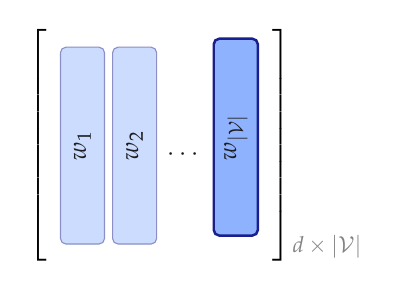
\begin{tikzpicture}
\matrix[matrix of nodes, left delimiter={[},right delimiter={]}, column sep=2.5pt,
        ampersand replacement=\&, nodes={colB}] (Wu) {
  \rotatebox{90}{$w_{1}$} \& \rotatebox{90}{$w_{2}$} \&
  |[draw=none,fill=none,minimum width=0.4cm]| $\cdots$ \& |[colBhi]| \rotatebox{90}{$w_{|\mathcal{V}|}$} \\ };
\node[font=\footnotesize, softgray, anchor=west] at ([xshift=5pt,yshift=2mm]Wu.south east) {$d \times |\mathcal{V}|$};
\end{tikzpicture}
\figcap{\textbf{$W_{\text{unembed}}$.} One column per vocabulary token. A representation is scored against all of them; the scores are the logits. (Often $W_{\text{embed}}^\top$.)}
\end{center}

There are $|\mathcal{V}|$ columns, one per vocabulary token, and for $j = 1, \ldots, |\mathcal{V}|$ the column $w_j \in \mathbb{R}^d$ is token $j$'s \textit{signature}: a pattern describing what a representation should look like for token $j$ to be the likely next word. Scoring a representation against all of them at once --- one dot product per column --- yields one number per token, the alignment of the representation with each signature, and these are the logits passed to the softmax.

A common and elegant choice ties these signatures to the input embeddings of Section~4. There, the embedding matrix $W_{\text{embed}}$ stored each token's vector as a \textit{row}; transposing it, $W_{\text{embed}}^\top$, stands those rows up as columns, and setting $W_{\text{unembed}} = W_{\text{embed}}^\top$ makes each token's output signature identical to its input embedding. This \textit{weight tying} saves a large number of parameters, since one matrix serves both ends, but it also says something meaningful: a token is predicted to the extent that the running representation has come to \textit{resemble that token's own embedding}. The model is, in effect, asking at each position which word the context now looks most like.

The scoring itself is one matrix multiplication.
\[
\text{logits} = X_{\text{final}}\, W_{\text{unembed}} \in \mathbb{R}^{n \times |\mathcal{V}|}, \qquad \text{logits}_{ij} = x_i^{\text{(final)}} \cdot w_j.
\]
Read through the measurement lens, entry $(i,j)$ is the alignment between position $i$'s representation and token $j$'s signature. Strong alignment yields a high score, meaning the model finds token $j$ a good fit for what position $i$ has come to mean. These raw scores are called \textit{logits}, and row $i$ holds one for every word in the vocabulary.

\subsubsection*{From Scores to Probabilities}

Logits are unbounded scores, not yet probabilities. Softmax, applied across each row, turns each row of logits into a probability distribution,

\begin{center}
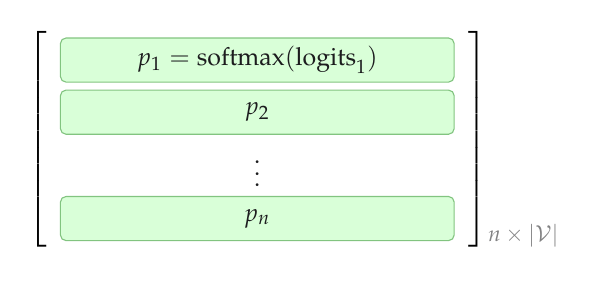
\begin{tikzpicture}
\matrix[matrix of nodes, left delimiter={[},right delimiter={]}, row sep=2.5pt, nodes={rowG, minimum width=5cm}] (P) {
  $p_{1}=\mathrm{softmax}(\text{logits}_1)$ \\ $p_{2}$ \\ |[draw=none,fill=none]| $\vdots$ \\ $p_{n}$ \\ };
\node[font=\footnotesize, softgray, anchor=west] at ([xshift=5pt,yshift=2mm]P.south east) {$n \times |\mathcal{V}|$};
\end{tikzpicture}
\figcap{\textbf{Output probabilities.} Each contextual representation is multiplied by $W_{\text{unembed}}$ to give $|\mathcal{V}|$ logits, then softmax turns row $i$ into a probability distribution over the next token.}
\end{center}
where $p_{ij}$ is the probability the model assigns to token $j$ following position $i$, and each row sums to one.

\subsubsection*{Training: Learning to Predict}

To train the model we need the right answer at each position, and the text already provides it. For every position but the last, the target $y_i$ is simply the token that follows it, read straight from the data with no labelling. Each such position is its own small prediction problem with its answer sitting inside the sequence, so one input of length $n$ supplies $n-1$ training signals.

Every position is therefore scored with the probability the model assigned to the token that actually followed. The cross-entropy loss records this,
\[
L_i = -\log P_{i, y_i},
\]
which is near zero when the model was confident and correct, since $P_{i,y_i}$ near one makes $-\log P_{i,y_i}$ near zero, and grows large when the model gave the true word little probability. Averaging over the $n-1$ predicting positions gives the loss for the whole sequence,
\[
L = -\frac{1}{n-1} \sum_{i=1}^{n-1} \log P_{i, y_i},
\]
and minimising it, across vast amounts of text, is the entire training objective. Every weight we have met, the embeddings, the projection matrices $W_Q$, $W_K$, $W_V$, the head mixer $W_O$, the feedforward weights, and the unembedding, is adjusted to make this number smaller.

\subsubsection*{Inference: Generating Text}

Given a prompt of $n$ tokens, we run a single forward pass, then look only at row $n$, the one position that has seen the entire prompt. Its distribution is the model's prediction for token $n+1$. We choose a token from it, append that token to the sequence, and run again, now with $n+1$ tokens, and repeat. 

The one freedom left is how to pick a token from each distribution, and several techniques exist. \textit{Greedy} decoding simply takes the single most likely token at every step, a fully deterministic choice. Sampling instead draws a token at random according to the distribution, and \textit{temperature} scaling tunes how that draw behaves by dividing the logits by a constant $T$ before the softmax. A low temperature, $T < 1$, sharpens the distribution and concentrates the draw on the model's favourites; a high temperature, $T > 1$, flattens it, raising the chance that less likely tokens are chosen and making generation more varied. Generation continues until the model emits the end-of-sequence token \texttt{<eos>}, reaches a length limit, or meets whatever other stopping rule the application sets.

\medskip

And there the journey closes. A sequence of token IDs entered as meaningless integers, became vectors carrying meaning and position, and passed through layers that alternately let each token gather context from the others and then process what it had gathered. Throughout, two readings of a single operation did the work, measurement asking how strongly one vector aligns with a learned direction, and mixing assembling each output as a recipe over learned components. At the very end, the same measurement reappears one last time, scoring each contextualised representation against the vocabulary to predict what comes next. Stack these blocks deep, train them on enough text, and from these few repeated parts what we are willing to call ``intelligence'' emerges.

\newpage
\bibliographystyle{plainnat}
\bibliography{main}

%==============================================================================
\appendix
% Appendix subsections stay out of the compact ToC so the contents still fit beneath
% the abstract on the title page.
\addtocontents{toc}{\protect\setcounter{tocdepth}{1}}
\newpage


%==============================================================================
%  APPENDIX STYLING  --- reuses the main preamble palette (ink / paper /
%  meas* blue family / mix* green family) so the video cards share the
%  visual language of the Section-2 diagrams and the hero callout box.
%==============================================================================

% Small palette-consistent chip (echoes the DRAFT chip on the title page).
\newcommand{\chip}[2][softgray]{%
  \tikz[baseline=-0.5ex]{\node[fill=#1, text=paper, rounded corners=2pt,
    inner xsep=4.5pt, inner ysep=1.8pt, font=\footnotesize\bfseries]{#2};}}

% "Watch" tag placed before each link (a play glyph in the section accent).
\newcommand{\watchtag}[1][measink]{%
  \tikz[baseline=-0.45ex]{%
    \node[fill=#1, text=paper, rounded corners=2pt,
      inner xsep=4pt, inner ysep=1.6pt, font=\scriptsize\bfseries]
      {$\blacktriangleright$\,\textsc{watch}};}}

% Thumbnail: a measdeep tile with a palette play button + duration chip,
% styled like the flat-architecture nodes (rounded corners=2pt).
% \vidthumb[<accent>]{<duration>}
\newcommand{\vidthumb}[2][measink]{%
  \begin{tikzpicture}
    \node[rounded corners=2pt, fill=measdeep, minimum width=2.95cm,
          minimum height=1.66cm, inner sep=0pt] (t) {};
    % subtle inner ring in the section accent
    \node[rounded corners=1.5pt, draw=#1!70, line width=0.5pt,
          minimum width=2.72cm, minimum height=1.42cm, inner sep=0pt] at (t.center) {};
    % play button: paper disc with an accent-colored triangle
    \node[circle, fill=paper, minimum size=0.66cm, inner sep=0pt] (pb) at (t.center) {};
    \fill[#1] ([xshift=0.02cm]pb.center) ++(-0.075cm,0.105cm)
      -- ++(0,-0.21cm) -- ++(0.185cm,0.105cm) -- cycle;
    % duration chip, bottom-right
    \node[anchor=south east, fill=ink!85, text=paper, rounded corners=1.5pt,
          inner xsep=3pt, inner ysep=1.3pt, font=\scriptsize\bfseries]
      at ([xshift=-3.5pt, yshift=3.5pt]t.south east) {#2};
  \end{tikzpicture}}

% Card container: the hero-callout idiom (hidden frame, ink!3!paper back,
% accent borderline). Single left accent by default.
% \begin{videobox}[<accent>] ... \end{videobox}
\newtcolorbox{videobox}[1][measink]{%
  enhanced, breakable, sharp corners,
  colback=ink!3!paper, frame hidden, boxrule=0pt,
  borderline west={2.5pt}{0pt}{#1},
  left=13pt, right=13pt, top=8pt, bottom=8pt,
  before skip=6pt, after skip=6pt}

% Capstone variant: blue-west / green-east double accent, matching the
% "Attention and the Feedforward Network" callout in Section 8.
\newtcolorbox{videoboxD}{%
  enhanced, breakable, sharp corners,
  colback=ink!3!paper, frame hidden, boxrule=0pt,
  borderline west={2.5pt}{0pt}{measink},
  borderline east={2.5pt}{0pt}{mixink},
  left=13pt, right=13pt, top=8pt, bottom=8pt,
  before skip=6pt, after skip=6pt}

% One video card. URLs are passed with RAW underscores; \nolinkurl handles
% them, so no manual escaping is needed.
% \vidcard[<accent>]{<duration>}{<title>}{<source>}{<description>}{<url>}
\newcommand{\vidcard}[6][measink]{%
  \begin{videobox}[#1]
  \noindent
  \begin{minipage}[c]{0.23\linewidth}\centering\vidthumb[#1]{#2}\end{minipage}%
  \hfill
  \begin{minipage}[c]{0.73\linewidth}
    \textbf{#3}\\[0.12em]
    {\small\itshape\color{softgray}#4}\\[0.5em]
    {\small #5}\\[0.55em]
    {\small\watchtag[#1]~\href{https://#6}{\textcolor{#1}{\nolinkurl{#6}}}}
  \end{minipage}
  \end{videobox}}

% Capstone card (double accent).
\newcommand{\vidcardD}[5]{%
  \begin{videoboxD}
  \noindent
  \begin{minipage}[c]{0.23\linewidth}\centering\vidthumb[measink]{#1}\end{minipage}%
  \hfill
  \begin{minipage}[c]{0.73\linewidth}
    \textbf{#2}\\[0.12em]
    {\small\itshape\color{softgray}#3}\\[0.5em]
    {\small #4}\\[0.55em]
    {\small\watchtag[measink]~\href{https://#5}{\textcolor{measink}{\nolinkurl{#5}}}}
  \end{minipage}
  \end{videoboxD}}

% Right-aligned runtime note, styled as a soft chip.
\newcommand{\runtime}[1]{%
  \par\vspace{0.4em}\noindent\hfill\chip[ink!55]{#1}}

%==============================================================================
\section{Prerequisites: Video Resources}
%==============================================================================

This appendix collects video resources for readers who want a thorough review of the mathematical foundations. The videos are organised into two sections.

%------------------------------------------------------------------------------
\subsection{Linear Algebra}
%------------------------------------------------------------------------------

The \textit{Essence of Linear Algebra} series by 3Blue1Brown provides geometric intuition for the concepts used throughout this document. The following chapters are particularly relevant:

\vidcard[measink]{9:52}{Vectors}{3Blue1Brown --- Essence of Linear Algebra, Ch.\ 1}{Introduces vectors as arrows in space and as lists of numbers. Establishes coordinates, vector addition, and scalar multiplication.}{youtube.com/watch?v=fNk_zzaMoSs}

\vidcard[measink]{9:59}{Linear combinations, span, and basis vectors}{3Blue1Brown --- Essence of Linear Algebra, Ch.\ 2}{Defines linear combinations as weighted sums of vectors. Introduces basis vectors and the idea that any vector can be built by scaling and adding basis vectors.}{youtube.com/watch?v=k7RM-ot2NWY}

\vidcard[measink]{10:59}{Linear transformations and matrices}{3Blue1Brown --- Essence of Linear Algebra, Ch.\ 3}{Shows that matrices encode linear transformations. The columns of a matrix tell you where the basis vectors land. Matrix--vector multiplication computes where a vector ends up after the transformation.}{youtube.com/watch?v=kYB8IZa5AuE}

\vidcard[measink]{14:12}{Dot products and duality}{3Blue1Brown --- Essence of Linear Algebra, Ch.\ 9}{Reveals the geometric meaning of the dot product: projecting one vector onto another and measuring the result. Connects dot products to linear transformations via duality.}{youtube.com/watch?v=LyGKycYT2v0}

\vidcard[measink]{16:45}{Abstract vector spaces}{3Blue1Brown --- Essence of Linear Algebra, Ch.\ 16}{Generalises vectors beyond arrows and lists of numbers. Shows that functions can be vectors too, and introduces the axioms that define a vector space. Explains why linear algebra applies to any setting with sensible notions of addition and scaling.}{youtube.com/watch?v=TgKwz5Ikpc8}

\runtime{Total runtime $\approx$ 1 hour}

%------------------------------------------------------------------------------
\subsection{Neural Networks}
%------------------------------------------------------------------------------

The following videos provide foundational knowledge on neural networks, including the concepts of parameterised functions, gradient descent, and backpropagation.

\vidcard[mixink]{18:40}{But what is a neural network?}{3Blue1Brown --- Deep Learning, Ch.\ 1}{Introduces neural networks as layered structures of neurons. Explains how weighted sums and activation functions combine to recognise patterns, using handwritten digit recognition as an example.}{youtube.com/watch?v=aircAruvnKk}

\vidcard[mixink]{20:33}{Gradient descent, how neural networks learn}{3Blue1Brown --- Deep Learning, Ch.\ 2}{Explains gradient descent as the process of iteratively adjusting weights to minimise a loss function. Visualises the loss landscape and the path towards better solutions.}{youtube.com/watch?v=IHZwWFHWa-w}

\vidcard[mixink]{12:47}{Backpropagation, intuitively}{3Blue1Brown --- Deep Learning, Ch.\ 3}{Builds intuition for backpropagation: how errors at the output propagate backward through the network to inform weight updates. Focuses on the conceptual picture rather than formulas.}{youtube.com/watch?v=Ilg3gGewQ5U}

\vidcard[mixink]{10:18}{Backpropagation calculus}{3Blue1Brown --- Deep Learning, Ch.\ 4}{Walks through the calculus of backpropagation: the chain rule applied layer by layer. Shows how gradients are computed in practice.}{youtube.com/watch?v=tIeHLnjs5U8}

\vidcard[mixink]{1:09:25}{MIT Introduction to Deep Learning | 6.S191}{Alexander Amini}{Covers perceptrons, activation functions, loss functions, gradient descent, backpropagation, and regularisation. Provides a comprehensive introduction to neural network foundations.}{youtube.com/watch?v=alfdI7S6wCY}

\runtime{Total runtime $\approx$ 2 hours 10 minutes ($\approx$ 1 hour excluding the MIT lecture)}

%==============================================================================
\newpage
\section{Further Resources: Large Language Models}
%==============================================================================

This appendix provides additional video resources for readers who want deeper context on LLMs and transformers. These videos by 3Blue1Brown offer visual explanations that complement the mathematical treatment in this document. 

\vidcardD{7:58}{Large Language Models explained briefly}{3Blue1Brown}{A concise overview of what LLMs are and how they work. Provides context for the detailed mechanics covered in this document.}{youtube.com/watch?v=LPZh9BOjkQs}

\vidcardD{27:14}{Transformers, the tech behind LLMs}{3Blue1Brown --- Deep Learning, Ch.\ 5}{Introduces the transformer architecture with visual animations. Covers embeddings, attention, and how information flows through the network.}{youtube.com/watch?v=wjZofJX0v4M}

\vidcardD{26:10}{Attention in transformers, step-by-step}{3Blue1Brown --- Deep Learning, Ch.\ 6}{A detailed walkthrough of the attention mechanism. Visualises how queries, keys, and values interact to route information between positions.}{youtube.com/watch?v=eMlx5fFNoYc}

\vidcardD{22:43}{How might LLMs store facts}{3Blue1Brown --- Deep Learning, Ch.\ 7}{Explores how factual knowledge might be encoded in transformer weights. Discusses the MLP layers as potential sites of fact storage and retrieval.}{youtube.com/watch?v=9-Jl0dxWQs8}

\runtime{Total runtime $\approx$ 1.5 hours}

\bigskip

\noindent\textbf{Further reading.} \textit{A Mathematical Framework for Transformer Circuits} \citep{elhage2021mathematical} extends this document's central ideas, developing the residual-stream view drawn in Figures~2a and~2b into a full framework for analysing what trained transformers compute.
%==============================================================================
%  APPENDIX C --- Stanford CS25: Transformers United (v6).  ENTIRELY NEW.
%  The section title and the prose are marked with \chg; the cards are not,
%  because ulem cannot be wrapped around tcolorbox/minipage content.
%==============================================================================
\newpage
\section{Further Resources: Stanford CS25 Transformers United}
%==============================================================================

CS25: Transformers United is a Stanford seminar series on transformer research, led in part by one of this document's authors and open to anyone, in person or by livestream. Each week a researcher working on the architecture gives a talk on their own work, and the recordings are made public. The sixth edition ran in the spring of 2026; its nine lectures are collected below, and the course pages are at \nolinkurl{web.stanford.edu/class/cs25}.

Where this document stays inside a single trained layer and derives it, these talks show what has been built around it: alternatives to the architecture, the engineering of training at scale, and the applications it now carries. They assume roughly what the preceding sections have supplied.

%------------------------------------------------------------------------------
\subsection{The Architecture and Its Alternatives}
%------------------------------------------------------------------------------

\vidcard[measink]{1:16:45}{Overview of Transformers}{Steven Feng \& Karan Singh --- Stanford University}{Opens the series with the history of machine learning and natural language processing, the transformer itself, and the impact it has had. Closes on recent trends, breakthroughs, applications, and the challenges that remain.}{youtube.com/watch?v=bHSDPgZYie0}

\vidcard[measink]{1:11:02}{From Representation Learning to World Modeling through Joint Embedding Predictive Architectures}{Hazel Nam \& Lucas Maes --- Brown University; Mila, Université de Montréal}{World models are moving away from reconstructing their input and towards predicting in a latent space instead. Presents two recent JEPA-based approaches that illustrate the shift from complementary angles.}{youtube.com/watch?v=GBd7iuJkW08}

\vidcard[measink]{1:17:07}{On the Tradeoffs of State Space Models and Transformers}{Albert Gu --- CMU and Cartesia AI}{A high-level overview of the state space model, a subquadratic alternative to the transformer. Covers the core characteristics and the design choices that separate SSMs from the architecture built up here.}{youtube.com/watch?v=OyimE74UMF8}

%------------------------------------------------------------------------------
\subsection{Training and Scale}
%------------------------------------------------------------------------------

\vidcard[mixink]{1:01:48}{The Ultra-Scale Talk: Scaling Training to Thousands of GPUs}{Nouamane Tazi --- Hugging Face}{Training a large language model takes more than raw compute; it takes a working understanding of parallelism and of the architectural choices that interact with it. Goes into the practicalities of training at ultra-scale.}{youtube.com/watch?v=I5BKi32IEa8}

\vidcard[mixink]{57:57}{From Next-Token Prediction to Next-Generation Intelligence: The Future of Pretraining}{Shrimai Prabhumoye --- Mistral AI, previously NVIDIA}{Recent progress in the design of pretraining algorithms. Emphasises the ordering of data, the integration of reasoning-centred data, and reinforcement-based objectives in shaping what a model can do.}{youtube.com/watch?v=e_H_tkpCAK4}

\vidcard[mixink]{1:12:30}{Distinct Modes of Generalization from Parameters and Context, and Paths to Bridge the Gap}{Andrew Lampinen --- Anthropic}{A model can be taught something by two routes: training on it, which updates the parameters, or presenting it in the context. Describes striking differences between the ways a model generalises from each, and how the gap might be closed.}{youtube.com/watch?v=dJtHauhRasc}

%------------------------------------------------------------------------------
\subsection{Applications and Systems}
%------------------------------------------------------------------------------

\vidcard[measink]{1:06:33}{Advancing Science and Medicine with Collaborative AI Agents}{Vivek Natarajan --- Google DeepMind}{Introduces general-purpose systems built to accelerate scientific discovery and widen access to medical expertise. Among them the AI co-scientist, a multi-agent Gemini-based system that generates and refines research hypotheses.}{youtube.com/watch?v=jFdH7n6BAl0}

\vidcard[measink]{1:04:40}{From Language Models to Native Multimodal Intelligence}{Victoria Lin --- Thinking Machines Lab}{Next-token prediction at scale induces remarkably general capabilities: acquiring knowledge, following instructions, reasoning and planning. Traces how the ideas behind language models have shaped multimodal ones, and where the next difficulties lie.}{youtube.com/watch?v=NDdc39KYqDU}

\vidcard[measink]{1:22:31}{Serving Transformers: Lessons from the Trenches of Production Inference}{Charles Frye --- Modal}{Training is only the first step in building an application. Turns to inference, forward passes without backward passes, and to what serving a model to real clients actually demands.}{youtube.com/watch?v=ZUdIsRZhWXI}

\bigskip

\noindent Five earlier editions of the series sit on the same channel, among them talks by Geoffrey Hinton, Ashish Vaswani and Andrej Karpathy.

%==============================================================================
%  APPENDIX D --- Karpathy's microgpt: the model as code.
%  code/microgpt_gpt.py is his gpt() verbatim from karpathy.github.io/2026/02/12/microgpt,
%  with a short comment block of ours at the top tying it to the document.
%==============================================================================
\newpage
\section{The Model as Code: Karpathy's microgpt}
%==============================================================================

\lstset{
  language=Python,
  basicstyle=\ttfamily\footnotesize\color{ink},
  keywordstyle=\color{measink}\bfseries,
  commentstyle=\color{softgray}\itshape,
  stringstyle=\color{mixdeep},
  showstringspaces=false,
  columns=fullflexible, keepspaces=true, tabsize=4, upquote=true,
  breaklines=true, breakatwhitespace=true,
  postbreak=\mbox{\textcolor{softgray}{$\hookrightarrow$}\space},
  backgroundcolor=\color{ink!3!paper},
  frame=l, framerule=2.5pt, rulecolor=\color{measink},
  xleftmargin=13pt, framexleftmargin=13pt, framesep=0pt,
  framextopmargin=6pt, framexbottommargin=6pt,
  aboveskip=18pt, belowskip=12pt,
}

This note took the transformer apart one matrix at a time. Andrej Karpathy's \textit{microgpt} puts it back together as code: a single file of about two hundred lines of plain Python, with no libraries, that trains a small GPT on a list of names and then samples new ones. Reproduced below is the function that defines the model, his code as written, with a few comments of ours at the top to tie it to this document. The complete runnable file, with the tokeniser, the tiny autograd engine, the training loop and the sampling loop, is in the post that accompanies it: \href{https://karpathy.github.io/2026/02/12/microgpt/}{\textcolor{measink}{\nolinkurl{karpathy.github.io/2026/02/12/microgpt}}}.

\lstinputlisting{code/microgpt_gpt.py}

\end{document}
